\documentclass[12pt,letter]{article}
\usepackage{mathptmx} % added for time new roman font
\usepackage[left=1in,right=1in,top=1in,bottom=1in]{geometry}
\usepackage[latin1]{inputenc}
\usepackage{amsmath}

% defines all example enviorment
\usepackage[framemethod=tikz]{mdframed} % added for the box around examples
\newtheorem{ex}{Example}
\numberwithin{ex}{section} % allows for the use of example numbers that lign up with the section numbers
\newenvironment{example}{\begin{mdframed}[middlelinewidth=0.5mm]\begin{ex}\normalfont}{\end{ex}\end{mdframed}}

% defines all review enviorment
\usepackage[framemethod=tikz]{mdframed} % added for the box around examples
\newtheorem{re}{Review}
\numberwithin{re}{section} % allows for the use of example numbers that lign up with the section numbers
\newenvironment{review}{\begin{mdframed}[middlelinewidth=2mm,roundcorner=20pt]\begin{re}\normalfont}{\end{re}\end{mdframed}}

% defines the quotation enviorment 
\usepackage{xcolor}
\newcommand{\quotebox}[2]{\begin{center}\fcolorbox{white}{blue!15!gray!15}{\begin{minipage}{0.9\linewidth}\vspace{10pt}\center\begin{minipage}{0.8\linewidth}{\space\Huge``}{#1}{\Huge''}{\break\null\hfill} {\small #2}  \end{minipage}\medbreak\end{minipage}}\end{center}}

% defines the definition enviorment 
\newcommand{\definitionbox}[2]{\begin{center}\fcolorbox{white}{blue!15!gray!15}{\begin{minipage}{0.9\linewidth}\vspace{10pt}\center\begin{minipage}{0.8\linewidth} {{\textbf{Definition} - }{#1}: {#2}}\end{minipage}\medbreak\end{minipage}}\end{center}}

\usepackage{amsfonts}
\usepackage{amssymb}
\usepackage{graphicx}
\usepackage{float}
\usepackage{booktabs}
%\usepackage{parskip} % remove all the paragraph indents

\usepackage{setspace}
%\usepackage[colorlinks=true]{hyperref}
\usepackage{textcomp} 
\usepackage{multicol} 


%%%%%%%		define the symbols for positive directions		%%%%%%
\makeatletter													%%	
																%%					
\newcommand*\curveplus{% positive counterclockwise				%%
  \mathbin{\rotatebox[origin=c]{90}{$\m@th\curvearrowleft$}+}}	%%
																%%
\newcommand*\rightplus{% positive right							%%
  \mathpalette\@rightplus\relax}								%%
\newcommand*\@rightplus[1]{%									%%
  \mathbin{\vcenter{\hbox{$\m@th\overset{#1+}{\to}$}}}}			%%
																%%	
\newcommand*\upplus{% positive up								%%
  \mathbin{+\mathord\uparrow}}									%%
																%%			
\newcommand*\downplus{% positive down							%%		
  \mathbin{+\mathord\downarrow}}								%%
  																%%		
\newcommand*\downrightplus{% positive down and right			%%	
  \mathbin{+ \rotatebox[origin=c]{-30}{$\m@th\rightarrow$}}}	%%
\makeatother 													%%	
%%%%%%%%%%%%%%%%%%%%%%%%%%%%%%%%%%%%%%%%%%%%%%%%%%%%%%%%%%%%%%%%%%


\usepackage{mathtools}          %loads amsmath as well added for the piece wise function
\DeclarePairedDelimiter\Floor\lfloor\rfloor
\DeclarePairedDelimiter\Ceil\lceil\rceil

 
\newcounter{NumberInTable}
\newcommand{\LTNUM}{\stepcounter{NumberInTable}{(\theNumberInTable)}}

\newcommand{\Laplace}[1]{\ensuremath{\mathcal{L}{\left[#1\right]}}}
\newcommand{\InvLap}[1]{\ensuremath{\mathcal{L}^{-1}{\left[#1\right]}}}
\renewcommand{\textuparrow}{$\uparrow$}

\begin{document}
	\large{}
	
	\setcounter{section}{1}
	\section{ Free Vibration of Single-Degree-of-Freedom Systems}






			
		Vibrations (i.e. the exchange of potential and kinetic energy) requires oscillatory motion that may repeat itself regularly or irregularly. A motion that is repeated on time intervals is called periodic motion. If this motion has a single frequency and amplitude it is called simple harmonic motion are represents the most basic form of oscillatory motion as depicted in figure \ref{fig:oscillatorymotion}.  For a 1-DOF system simple harmonic motion is defined as a periodic motion where the restoring force is directly proportional to the displacement and acts in the direction opposite to that of displacement.	
		

		\begin{figure}[H]
			\centering
			\includegraphics[]{../figures/oscillatory_motion.png}
			\caption{Oscillatory motion for a single degree of freedom system showing (a) periodic motion; and (b) simple harmonic motion.}
			\label{fig:oscillatorymotion}
		\end{figure}

		Given the nature of simple harmonic motion, constant amplitude and frequency, the wave starting at the origin $O$ can be modeled at a point on the end of a vector with length $A$ rotating rotating at a constant angular velocity $\omega_n$ where the angle from the origin of the vector is $\phi$, defined as $\phi = \omega t$. Where $\omega$ is the lowercase Greek letter Omega and $\phi$ is the lowercase Coptic letter phi. This is similar to a Greek phi ($\varphi$) and either can be used in this context. The subscript $n$ on $\omega$ denotes that this frequency relates to the natural frequency of the system, the only frequency in simple harmonic motion. A visualization of the harmonic motion obtained from projecting the point on the edge of a vector onto the $\omega_n t$ space is presented in figure \ref{fig:Harmonic_Motion}. 

		\begin{figure}[H]
			\centering
			\includegraphics[]{../figures/harmonic_motion.png}
			\caption{Harmonic motion represented at the projection of a point on the end of a vector moving on a circle. Note the axis $\omega_n t$.}
			\label{fig:Harmonic_Motion}
		\end{figure}

	\subsection{Mathematical Modeling of Free Vibration}

		The Development of a mathematical model for a system under free vibration would enable the practitioner to predict, or model, the vibrating system of interest.  Therefore, considering that the following system, 
		
		\begin{figure}[H]
			\centering
			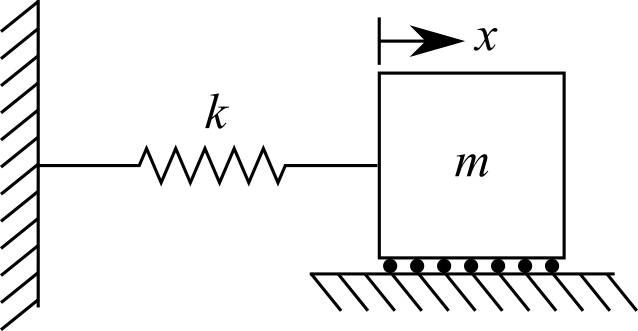
\includegraphics[]{../figures/1-DOF-spring_mass_horizontal.png}
			\caption{1-DOF spring-mass system.}
		\end{figure}
		\noindent can be modeled expressed with the following EOM
		\begin{equation}
			m\ddot{x}(t) + kx(t) = 0
			\label{eq:EOM}
		\end{equation}		
		it becomes prudent to solve this homogeneous ordinary differential equation (ODE) to obtain a model of the vibrating system. The simplest method for solving an ODE is to propose a solution based on observations of a vibrating physical system. Figure \ref{fig:Harmonic_Motion_2.png} reports and annotates the key components from an observation of a vibrating system. 
		
		\begin{figure}[H]
			\centering
			\includegraphics[]{../figures/harmonic_motion_2.png}
			\caption{Summary of the temporal response for a 1-DOF system.}
			\label{fig:Harmonic_Motion_2.png}
		\end{figure}
		\noindent where $x_0$ and $v_0$ are the is the displacement and velocity at $t$=0 (i.e. the initial displacement). 
				

		A mathematical expression can now be formulate to represent the observed simple harmonic motion. This expression can be based on the projection of a point on a vector (transposed into the time domain) or assembled from constituent parts as done in what follows. Solving for a location $x$, at a time $t$; $x(t)$, the various characteristics of the expression can be identified:

		\subsubsection{Solve for the Natural Frequency ($\omega_n$) of the System }
				
			\begin{itemize}
				\item System oscillates $\rightarrow$ a sin function models this 
				\item System oscillates at different speed $\rightarrow$ use a parameter to adjust $\omega_n$ in rad/s. 
				\item Systems have different amplitudes $\rightarrow$ use a parameter to adjust $A$ in meters.
				\item System has different starting points $\rightarrow$ use a parameter to adjust $\phi$ in rad. 
			\end{itemize}

			\noindent Using these four constituent components, an equation can be proposed: 
			\begin{equation}
				{x}(t) = A\text{sin}(\omega_n t + \phi)
			\end{equation}
			Take the derivative to get velocity:
			\begin{equation}
				\dot{x}(t) = A\omega_n\text{cos}(\omega_n t + \phi)
			\end{equation}
			Take the derivative again to get acceleration:
			\begin{equation}
			\ddot{x}(t) = -A\omega_n^2\text{sin}(\omega_n t + \phi)
			\end{equation}
			Substituting $x$ and $\ddot{x}$ into the EOM for the considered 1-DOF system ($m\ddot{x}(t) + kx(t) = 0$) yields:
			\begin{equation}
				m\big(-A\omega_n^2\text{sin}(\omega_n t + \phi)\big) + k\big(A\text{sin}(\omega_n t + \phi)\big) = 0
			\end{equation}
			Thereafter, dividing both sides by $A\text{sin}(\omega_n t + \phi)$ results in the expression:
			\begin{equation}
				-m\omega_n^2+k = 0
			\end{equation}
			This expression can be rearranged into the more useful standard form:
			\begin{equation}
				\omega_n= \sqrt{\frac{k}{m}}
				\label{eq:natural_frequency}
			\end{equation}
			Equation \ref{eq:natural_frequency} represents a solution to the EOM  presented in equation \ref{eq:EOM}. This solution is not in the form of an ODE  so, therefore, we can experientially prove that this is the correct solution. For example, we could build a systems with known mass and stiffness and measure the natural frequency of the system. Equation \ref{eq:natural_frequency} equation leads to:
			\begin{equation}
				T= \frac{2 \pi}{\omega_n}
			\end{equation}
			where $T$ is the period of oscillations and 
			\begin{equation}
				f_n= \frac{\omega_n}{2 \pi}
			\end{equation}
			where $f_n$ is the frequency of the oscillations. 
					
		\subsubsection{Solve for Initial Phase ($\phi$) of the System }
			The EOM is a second-order ODE so there needs to exist two initial conditions (constants) to solve it. For the systems under considerations, the displacement ($x$) and velocity ($\dot{x}$ or $v$) at $t=0$ are the initial conditions. For simplicity, these are written as 
			\begin{equation}
				x(0) = x_0  
			\end{equation}			
			\begin{equation}
				\dot{x}(0) = v(0) = v_0 
			\end{equation}			
			Setting the equation to its initial state $t=0$, the equations for displacement and velocity can be simplified to: 
			\begin{equation}
				{x}(0) = x_0 = A\text{sin}(\omega_n 0 + \phi) = A\text{sin}(\phi)
				\label{eq:x_0=Asintheta} 
			\end{equation}
			\begin{equation}
				\dot{x}(0) = v_0 = A\omega_n\text{cos}(\omega_n0 + \phi) = A\omega_n\text{cos}(\phi)
				\label{eq:v_0=Aomegacosphi} 
			\end{equation}
			Thereafter, mathematical meanings for $\phi$ and $A$ can be derived. To do this, $\phi$  can be solved for by rearranging equations \ref{eq:x_0=Asintheta} and \ref{eq:v_0=Aomegacosphi} for $A$:
			\begin{equation}
				A = \frac{x_0}{\text{sin}(\phi) }
			\end{equation}
			and:
			\begin{equation}
				A = \frac{v_0}{\omega_n\text{cos}(\phi)}
			\end{equation}
			Setting these two equations equal to each other cancels out A and creates:
			\begin{equation}
				\frac{x_0 \omega_n}{\text{sin}(\phi)} = \frac{v_0}{\text{cos}(\phi)} 
			\end{equation}
			therefore:
			\begin{equation}
				\frac{x_0\omega_n}{v_0} = \frac{\text{sin}(\phi)}{\text{cos}(\phi)}
			\end{equation}
			finally:
			\begin{equation}
				\phi = \text{tan}^{-1}\bigg(\frac{x_0\omega_n}{v_0}\bigg)
			\end{equation}
			
		\subsubsection{Solve for Amplitude ($A$) of the System }
			
			The amplitude of the vibrating system ($A$) is solved for in a similar manner to $\phi$ where the expressions for $x$ and $\dot{x}$ are solved for at $t=0$ and rearranged as to isolate $\phi$. This operations results in the the equations:  
			\begin{equation}
				\text{sin}(\phi) = \frac{x_0}{A}
			\end{equation}
			and:
			\begin{equation}
				\text{cos}(\phi) = \frac{v_0}{\omega_nA}
			\end{equation}
			From these equations a value for $\phi$ can be obtained knowing that $\text{sin}(\phi)^2+\text{cos}(\phi)^2=1$. Therefore:
			\begin{equation}
				\bigg(\frac{x_0}{A}\bigg)^2  + \bigg(\frac{v_0}{\omega_nA}\bigg)^2 = 1
			\end{equation}
			multiplying each expression by 1 (also expressed as $\frac{\omega_n}{\omega_n}$), gives the equation:
			\begin{equation}
				\bigg(\frac{\omega_n}{\omega_n}\bigg)^2\bigg(\frac{x_0}{A}\bigg)^2  + 1 \bigg(\frac{v_0}{\omega_nA}\bigg)^2  = 1 \times 1
			\end{equation}
			which becomes:
			\begin{equation}
				\bigg(\frac{\omega_n x_0}{\omega_n A}\bigg)^2  + \bigg(\frac{v_0}{\omega_nA}\bigg)^2 = 1
			\end{equation}
			Further simplification is obtained by multiplying each side by $(\omega_n A)^2$ to obtain:
			\begin{equation}
				\omega_n^2x_0^2+v_0^2=A^2\omega_n^2 
			\end{equation}
			Solving for $A$, this expression rearranges to:
			\begin{equation}
				A = \frac{\sqrt{\omega_n^2x_0^2+v_0^2}}{\omega_n} = \sqrt{x_0^2+\bigg(\frac{v_0}{\omega_n}\bigg)^2}
			\end{equation}
		
		\subsubsection{Response for Simple Harmonic Motion}
			
			The time-varying displacement of a 1-DOF vibrating system under free response is expressed by the equation ${x}(t) = A\text{sin}(\omega_n t + \phi)$. Substituting in the expressions for $A$ and $\phi$ results in:
			
			\begin{equation}
				{x}(t) = \frac{\sqrt{\omega_n^2x_0^2+v_0^2}}{\omega_n}\text{sin}\Bigg(\omega_n t + \bigg( \text{tan}^{-1}\bigg(\frac{x_0\omega_n}{v_0}\bigg)\bigg)\Bigg)
				\label{eq:response_simple_harmonic_motion}
			\end{equation}
			
			\noindent This equation provides a mathematical solutions that relates displacement of the mass to the initial conditions $x_0$ and $v_0$. The solution is considered a free response because no input is applied after t=0. The relationship between the initial conditions ($x_0$ and $v_0$) and the amplitude and phase of the response can be expressed using the Pythagorean theorem, $a^2 + b^2 = c^2$, as annotated in figure \ref{fig:Trigonometric_relationship}.
			
			\begin{figure}[H]
				\centering
				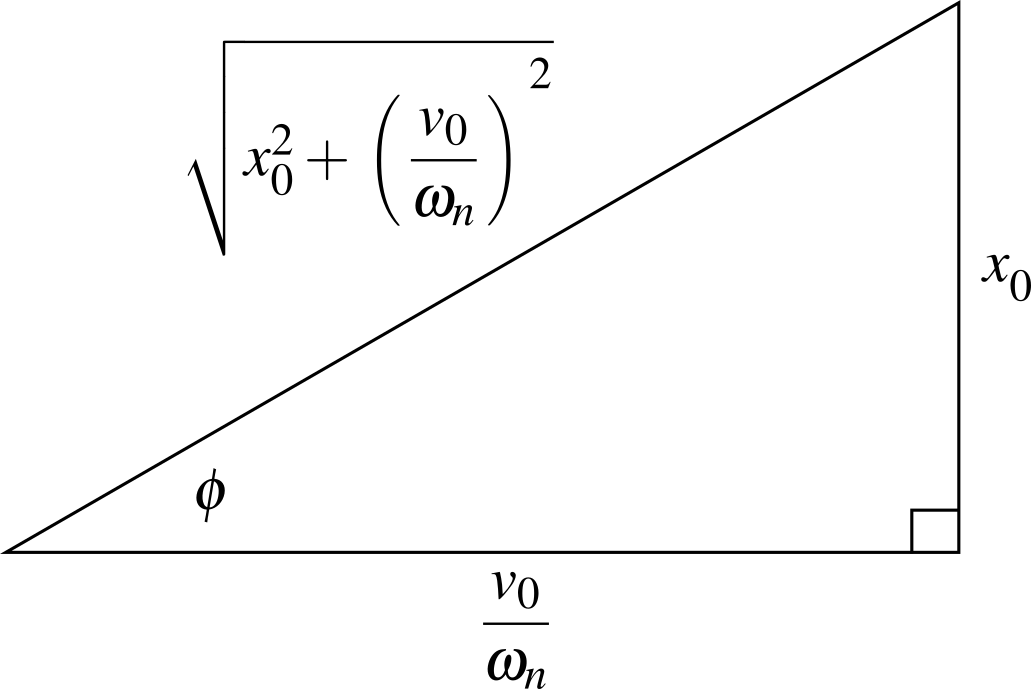
\includegraphics[]{../figures/trigonometric_relationship_undamped_free.png}
				\caption{Trigonometric relationship between the initial conditions ($x_0$ and $v_0$), amplitude $A$, and phase $\phi$ for free vibration of a 1-DOF system.}
				\label{fig:Trigonometric_relationship}
			\end{figure}

		\subsubsection{Special Considerations for No Initial Velocity ($v_0=0$)}
		
			Upon close inspection of the temporal solution in equation \ref{eq:response_simple_harmonic_motion}, it becomes evident that any system without initial velocity (i.e. $v_0=0$) results in an undefined number for $(x_0\omega_n)/v_0$. A solution to this challenge lies in the fact that limit of tan$^{-1}(x)$ approaches $-\pi/2$ at $-\infty$ and  $\pi/2$ at $\infty$, as depicted in figure \ref{fig:arctan_plot}. Therefore, the solution at $-\infty$ and $\infty$ is undefined, resulting in the expression:
			
			\begin{equation}
				\bigg(\frac{x_0\omega_n}{v_0}\bigg) = \pm \frac{\pi}{2}, \text{ when } v_0=0
			\end{equation}			
			
			This step is applied in IEEE floating point arithmetic (IEEE 754) and results in either $\pi/2$ or $\pm \pi/2$ depending on the rounding format used. From the practitioner's side, it becomes important to recognize the situation $v_0=0$ and correct this value as needed. 
			
			\begin{figure}[H]
				\centering
				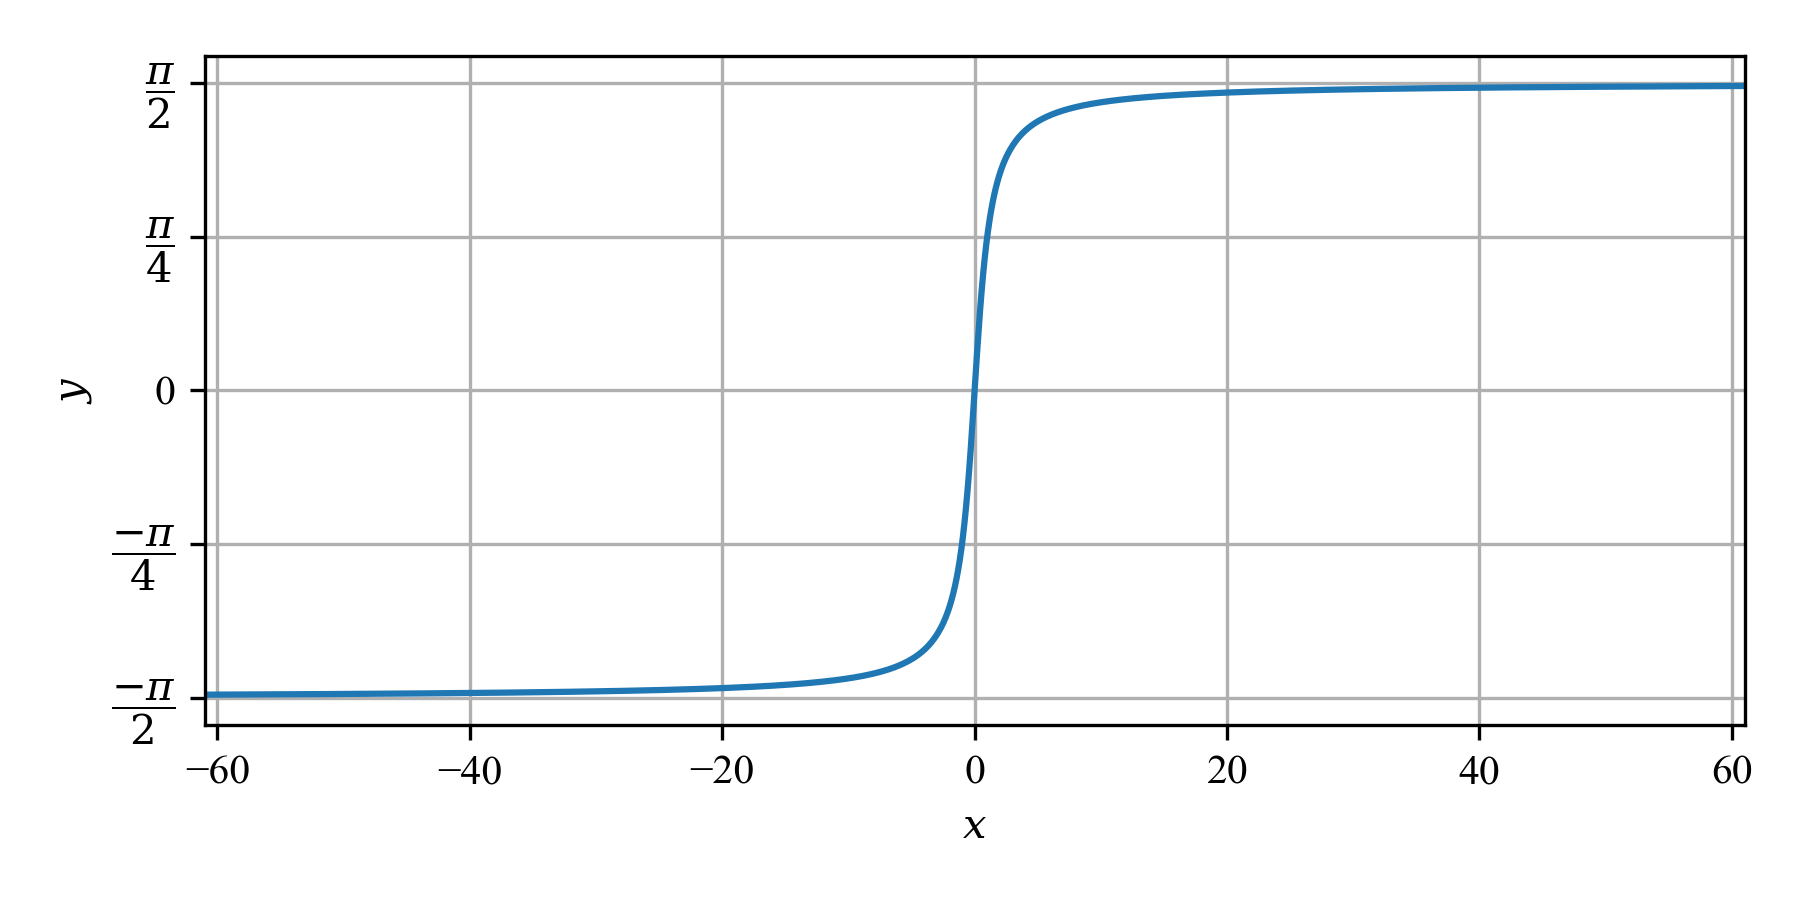
\includegraphics[]{../figures/arctan_plot.png}
				\caption{Response of tan$^{-1}$ (or arctan) for  $x$=-60 to 60 showing that the tan$^{-1}$ is undefined as $x$ approaches $-\infty$ and $\infty$.}
				\label{fig:arctan_plot}
			\end{figure}		
			

			\begin{example}
		
				A vehicle wheel, tire, and suspension can be modeled as a SDOF spring and mass as depicted below: The mass of the wheel and tire is measured to be 300 kg and its frequency of oscillation is observed to be 10 rad/sec. What is the stiffness of the wheel assembly?
				
				\begin{figure}[H]
					\centering
					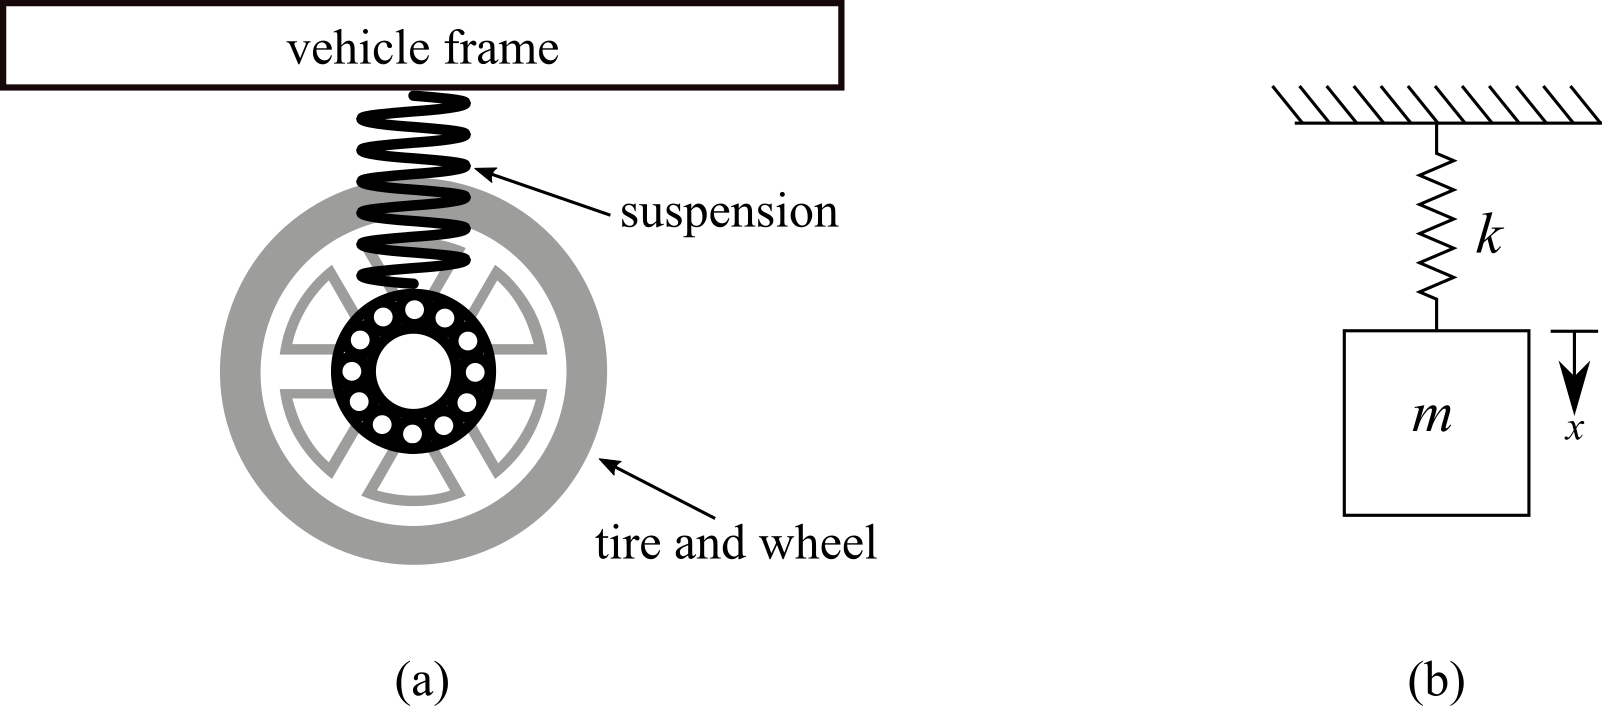
\includegraphics[]{../figures/Vehicle_wheel_undamped.png}
					\caption{Modeling of a vehicle wheel, tire, and suspension showing: (a) Graphical representation; and (b) a spring-mass model.}
					\label{fig:vehicle_wheel_undamped}
				\end{figure}				
				
				\noindent\textbf{Solution:} 
				Considering:
				\begin{equation}
					\omega_n = \sqrt{\frac{k}{m}}
				\end{equation}
				therefore, $k=m\omega_n^2=(300$ $\text{kg})(10$ $\text{rad/s})^2=30$ KN/m. Note: radians are a dimensionless quantity and as such the units of  $m\omega_n^2$ become  $\frac{\rm{kg}}{\rm{s}^2}\cdot\frac{\rm{m}}{\rm{m}}$ where the unit value $\frac{\rm{m}}{\rm{m}}$ is added such that the stiffness of the spring can be expressed as $\frac{\rm{kg}\cdot \rm{m}}{\rm{s}^2}\cdot\frac{1}{\rm{m}}$ = $\frac{\rm{N}}{\rm{m}}$.
			\end{example}
			
			\begin{example}		
				Consider the following 1-DOF system, where $k = 857.8$ N/m and $m=49.2\times10^{-3}$ kg, calculate the natural frequency in rad/s and Hz. Also find the period of oscillations and the maximum displacement if the spring is initially displaced $10$ mm with no initial velocity.  	
				\begin{figure}[H]
					\centering
					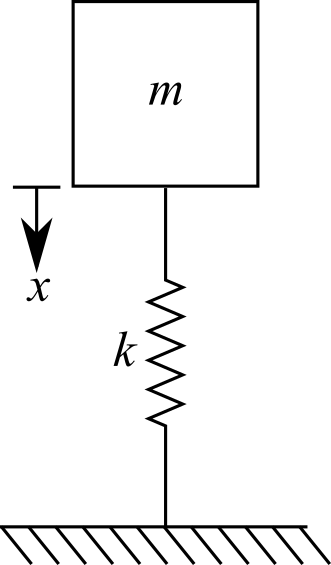
\includegraphics[]{../figures/1-DOF-mass_vertical.png}
					\caption{1-DOF spring-mass system.}
				\end{figure}		
	
				\noindent\textbf{Solution:} 
				\begin{equation}
					\omega_n = \sqrt{\frac{k}{m}}= \sqrt{\frac{857.8}{49.2\times10^{-3}}} = 132 \hspace{1ex}\text{rad/sec}
				\end{equation}	
				In Hz, this is:
				\begin{equation}
					f_n = \frac{\omega_n}{2\pi} = 21 \hspace{1ex}\text{Hz}
				\end{equation}						
				The period is:
				\begin{equation}
					T = \frac{2\pi}{\omega_n} = 0.0476 \hspace{1ex}\text{s}
				\end{equation}					
				The maximum displacement will happen when sin($\omega_nt+\phi$)$=0$, therefore, the value of $A$ is the maximum displacement. For an undamped system, $	A = \frac{\sqrt{\omega_n^2x_0^2+v_0^2}}{\omega_n}$,  
	
	
				\begin{equation}
					A = \frac{\sqrt{\omega_n^2x_0^2+v_0^2}}{\omega_n} = \frac{\sqrt{132^2 0.01 ^2+0^2}}{132}=0.01 \hspace{1ex}\text{m}
				\end{equation}
	
			\end{example}

	\subsection{General Solution for Vibrating Systems}

		The EOM for a vibrating system has many solutions and can be be expressed in various forms including a general solution. These forms offer different mathematical approaches to solve the same 1-DOF spring-mass system and relate to each other through Euler's equations.
				
		\begin{review}
			Vibration analysis uses complex numbers to solve the EOM's differential equation. In this text the imaginary number is termed $j$ (sometimes referred to as $i$): such that:
			
			\begin{equation}
				j = \sqrt{-1}
			\end{equation}		
			and:	 
			\begin{equation}
				j^2 = -1
			\end{equation}	
			A general complex number, $x$, can be expressed as:
			\begin{equation}
				x=a+bj
			\end{equation}			 	
			here, $a$ is referred to as the real number and $b$ is the imaginary part of the number $x$. Such complex numbers can be represented in the complex plane, also called a Argand plot. The absolute value or modules is defined as $|x|$ presented on the complex plot. 
			
			\begin{figure}[H]
				\centering
				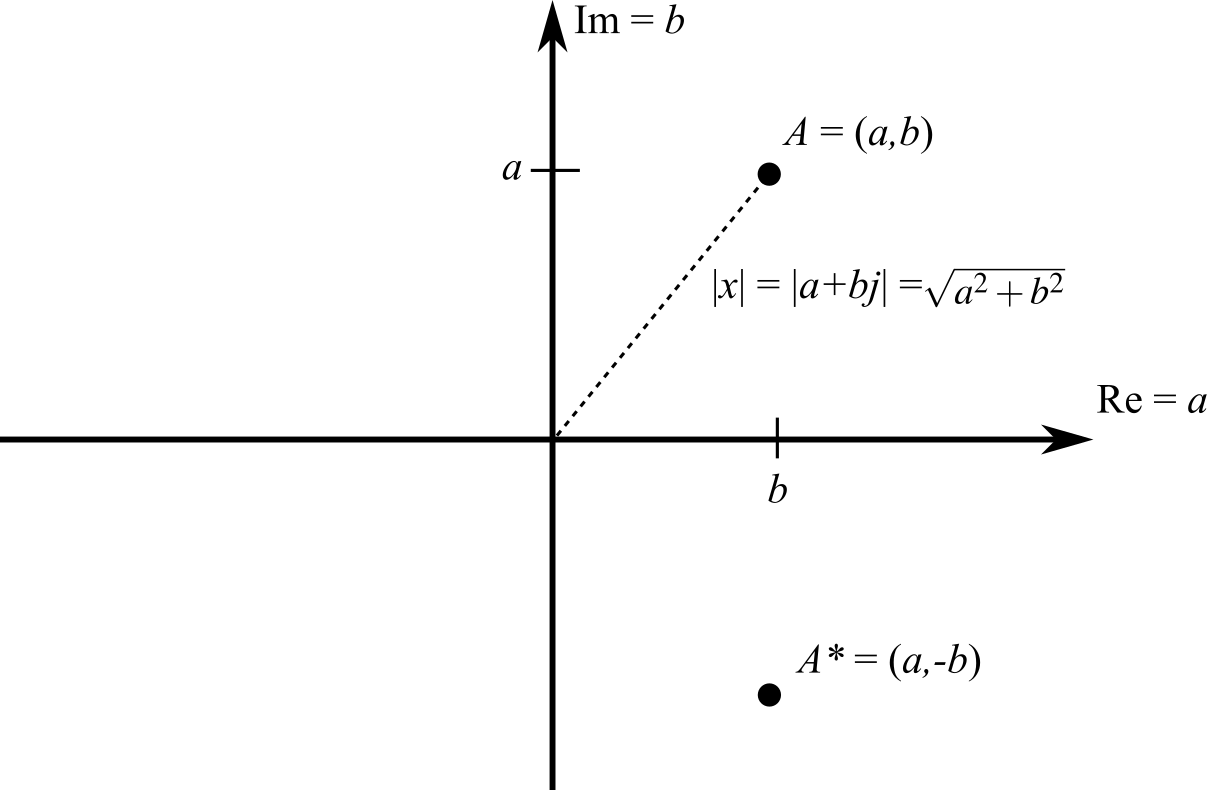
\includegraphics[]{../figures/complex_plane.png}
				\caption{A conjugate pair of numbers ($A$ and $A*$) represented on the complex plane.}
			\end{figure}
					
			$A$ and $A^*$ prime are complex conjugate pairs. In mathematics, the complex conjugate of a complex number is the number with an equal real part and an imaginary part equal in magnitude but opposite in sign. In other words, a conjugate pair is $a + bj$ and $a - bj$.  
			
			\definitionbox{con�ju�gate (adjective)}{Coupled, connected, or related.}

		\end{review}			
		\begin{review}
		
			Euler's (pronounced oy-ler) formula, named after Swiss engineer and mathematician Leonhard Euler (1707-1783), is a mathematical formula in complex analysis that establishes the fundamental relationship between the trigonometric functions and the complex exponential function. Euler's formula states that for any real number $x$,
			\begin{equation}
				e^{j\psi} = \text{cos}(\psi) + j \text{sin}(\psi)
			\end{equation}		
			where $j=\sqrt{-1}$. This equation can also be expressed as:
			\begin{equation}
				e^{-j\psi} = \text{cos}(\psi) - j \text{sin}(\psi)
			\end{equation}	
			This can be expressed in terms of polar coordinates as:				
			\begin{figure}[H]
				\centering
				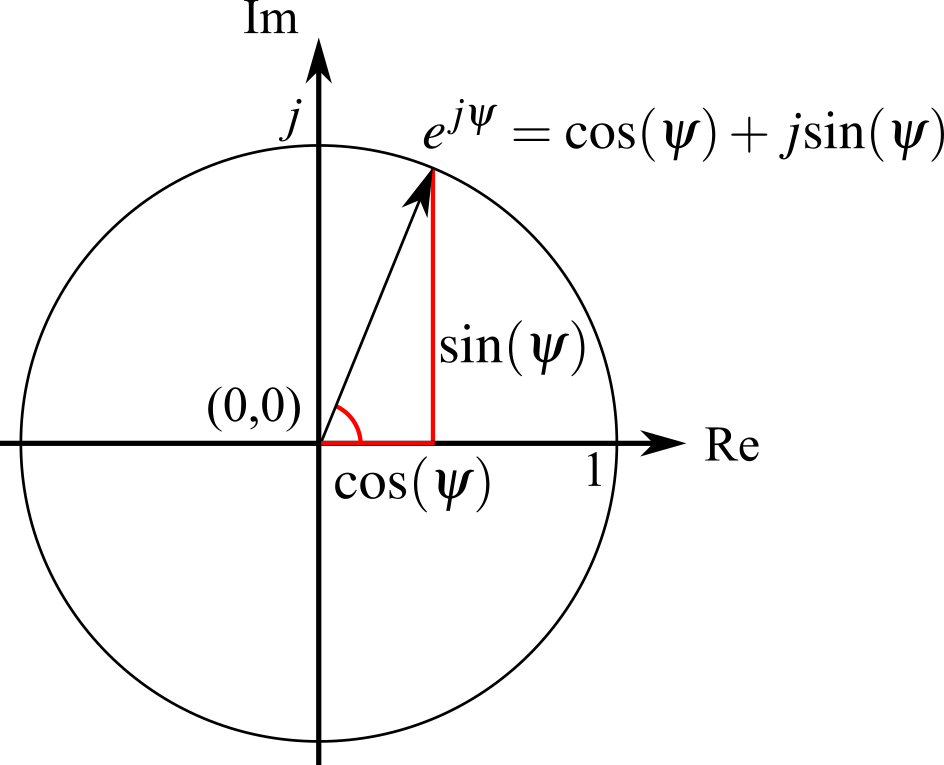
\includegraphics[]{../figures/Eulers_formula.png}
				\caption{Euler's formula illustrated on the unit circle in the complex plane.}
			\end{figure}
		\end{review}
		
		\subsubsection{Formulating the General Solution for a 1-DOF Spring-Mass System}
			We can also solve the following EOM as an elementary differential equation:
			\begin{equation}
				m\ddot{x}+kx=0
			\end{equation}		
			in a more analytical manner using the theory of elementary differential equations. To do this is the form: 
			\begin{equation}
				x(t) = ae^{\lambda t}
			\end{equation}
			is assumed where, $a$ and $t$ are nonzero constants that need to be determined. Using successive differentiation,the assumed solution becomes:
			\begin{equation}
				\dot{x}(t) = \lambda ae^{\lambda t}
			\end{equation}
			and 
			\begin{equation}
				\ddot{x}(t) = \lambda^2 ae^{\lambda t}
			\end{equation}
			therefore, $m\ddot{x}(t) + kx(t) = 0$ becomes:
			\begin{equation}
				m \lambda^2 ae^{\lambda t}  + k ae^{\lambda t} = 0
			\end{equation}
			Next, the above expressions is divide by $ae^{\lambda t}$ to obtain the characteristic equation:
			\begin{equation}
				m \lambda^2 + k = 0
			\end{equation}
			This can be done because $ae^{\lambda t}$ is never zero, therefore, the expressions is never divide by zero. The quadratic formula gives us:
			\begin{equation}
				\lambda = \pm \sqrt{-\frac{k}{m}} = \pm \sqrt{\frac{k}{m}}j = \pm \omega_n j
			\end{equation} 
			remember that $\omega_n = \sqrt{\frac{k}{m}}$. Notice that the $\pm$ tells us there are two solutions to this problem. So, putting $\lambda$ back into the assumed solution results in two solutions (one positive, one negative):   
			\begin{equation}
				x(t) = a_1e^{+\omega_n j t}
			\end{equation}
			and 
			\begin{equation}
				x(t) = a_2e^{-\omega_n j t}
			\end{equation}
			As these solutions only consider, and are only valid for, linear systems, the sum of the solutions is also a solution. This simplification results in:
			\begin{equation}
				x(t) = a_1e^{+\omega_n j t} + a_2e^{-\omega_n j t}
			\end{equation}
			where $a_1$ and $a_2$ are complex valued constants of integration.
			
			\begin{example}
				Show that $	x(t) = a_1e^{+\omega_n j t} + a_2e^{-\omega_n j t}$ is equal to $A\text{sin}(\omega_n+\phi)$. \\
				
				\noindent\textbf{Solution:} 
				This equation was derived using Euler's formula and it can be shown that this equation is equivalent to the $A\text{sin}(\omega_n+\phi)$. To recover the previously assumed solution, the knowledge that $a_1$ and $a_2$ are complex congregate pairs and as such the magnitude can be expressed as $a_1=a_2$ is leveraged. Using Euler's polar notation, $a_1$ and $a_2$ can be expressed as 
				\begin{equation}
					a_1 = a_2 = ae^{j\psi}
				\end{equation}	
				where $a$ and $\psi$ are real numbers, the equation becomes:		
				\begin{equation}
					x(t) = ae^{j(\omega_n t+\psi)} + ae^{-j(\omega_n t+\psi)}
				\end{equation}			
				this becomes:
				\begin{equation}
					x(t) = a(e^{j(\omega_n t+\psi)} + e^{-j(\omega_n t+\psi)})
				\end{equation}				
				Remembering Euler's equations from before, this becomes:
				\begin{equation}
					x(t) = a\big(\text{cos}(\omega_n t+\psi) + j \text{sin}(\omega_n t+\psi) + \text{cos}(\omega_n t+\psi) - j \text{sin}(\omega_n t+\psi)\big)
				\end{equation}				
				combining the ``cos'' terms and canceling out the ``sin'' terms this becomes:
				\begin{equation}
					x(t) = 2a \cdot \text{cos}(\omega_n t+\psi)
				\end{equation}						
				This is equivalent to $	{x}(t) = A\text{sin}(\omega_n t + \phi)$ considering that $A=2a$ and knowing sin($\phi$) = cos($\phi + \psi$). To expand, this is because the sin and cos are only differentiated by a phase shift. 			
			\end{example}

			
			Next, a general solution for the EOM is obtained. Using the previous solution:
			\begin{equation}
				x(t) = a_1e^{+\omega_n j t} + a_2e^{-\omega_n j t}
			\end{equation}			
			we can expand this into the form: 
			\begin{equation}
				x(t) = a_1\big(\text{cos}(\omega_n t) + j \text{sin}(\omega_n t)\big) + a_2\big(\text{cos}(\omega_n t) - j \text{sin}(\omega_n t)\big)
			\end{equation}
			using trigonometric functions. This equates to:
			\begin{equation}
				x(t) = (a_1+a_2) \cdot \text{cos}(\omega_n t) + (a_1-a_2)j \cdot \text{sin}(\omega_n t)
			\end{equation}			
			As $x(t)$ is always real, $A_1$ and $A_2$ can be defined as:
			\begin{equation}
				A_1 = (a_1+a_2)
			\end{equation}		
			and
			\begin{equation}
				A_2 = (a_1-a_2)j
			\end{equation}	
			Lastly, as the general solution is written as:
			\begin{equation}
				x(t) = A_1\text{cos}(\omega_n t) + A_2\text{sin}(\omega_n t)
			\end{equation}	
			This is the general solution for the EOM ($m\ddot{x}+kx=0$) of the considered oscillating system where $A_1$ and $A_2$ are defined as:
			\begin{equation}
				A = \sqrt{A_1^2+ A_2^2}
			\end{equation}
			and	
			\begin{equation}
				\phi = \text{tan}^-1\bigg(\frac{A_1}{A_2}\bigg)
			\end{equation}		
			These are obtained from a trigonometric relationship, similar to that used before:
			\begin{figure}[H]
				\centering
				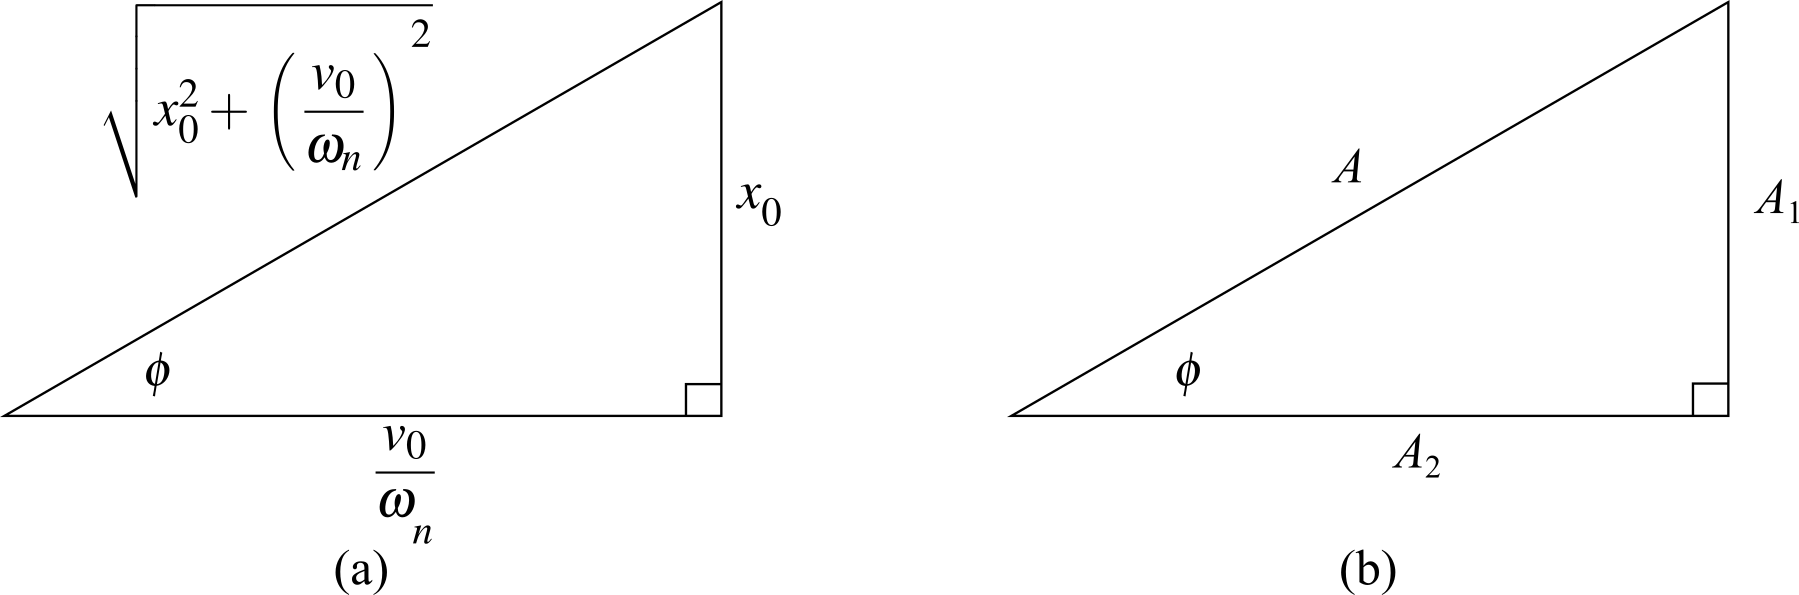
\includegraphics[]{../figures/trigonometric_relationship_undamped_free_general_solution.png}
				\caption{Trigonometric relationship between the initial conditions, amplitude, and phase, for free vibration of a 1-DOF system expressed with: (a) variables for initial conditions; and (b) generic variables $A_{1}$ and $A_{2}$.}
			\end{figure}
			\noindent again, $A$ and $\phi$ are:
			\begin{equation}
				A = \frac{\sqrt{\omega_n^2x_0^2+v_0^2}}{\omega_n} = \sqrt{x_0^2+\Bigg(\frac{v_0}{\omega_n}\Bigg)^2}
			\end{equation}
			\begin{equation}
				\phi = \text{tan}^{-1}\bigg(\frac{x_0\omega_n}{v_0}\bigg)
			\end{equation}		


			\begin{example}			
				Using the general solution: 
				\begin{equation}
					x(t) = A_1\text{cos}(\omega_n t) + A_2\text{sin}(\omega_n t)
				\end{equation}			
				Calculate the values of $A_1$ and $A_2$ in terms of their initial conditions $x_0$ and $v_0$.
				
				\noindent\textbf{Solution:} Knowing the following for $x$ and $\dot{x}$:
				\begin{equation}
					x(t) = A_1\text{cos}(\omega_n t) + A_2\text{sin}(\omega_n t)
				\end{equation}	
				\begin{equation}
					\dot{x}(t) = -A_1\omega_n\text{sin}(\omega_n t) + A_2\omega_n\text{cos}(\omega_n t)
				\end{equation}	
				Now apply the initial conditions, $x(0)=0$ and $v(0)=0$, this yields:
				\begin{equation}
					x(0) = x_0 = A_1
				\end{equation}	
				\begin{equation}
					\dot{x}(0)= v_0  =  A_2\omega_n
				\end{equation}
				Solving for $A_1$ and $A_2$ shows us:
				\begin{equation}
					A_1 = x_0 \text{, and } A_2 = \frac{v_0}{\omega_n}
				\end{equation}
				thus:
				\begin{equation}
					x(t) = x_0\text{cos}(\omega_n t) + \frac{v_0}{\omega_n}\text{sin}(\omega_n t)
				\end{equation}				
			\end{example}

		\subsubsection{Solution of 1-DOF System in Three Forms}
			Form one, for $m\ddot{x} + kx =0$ subject to nonzero initial conditions can be written as:  		
			\begin{equation}
				x(t) = a_1e^{+\omega_n j t} + a_2e^{-\omega_n j t}
			\end{equation}	
			where $a_1$ and $a_2$ are complex terms. Form two is:
			\begin{equation}
				{x}(t) = A\text{sin}(\omega_n t + \phi)
			\end{equation}
			while form three is:
			\begin{equation}
				x(t) = A_1\text{cos}(\omega_n t) + A_2\text{sin}(\omega_n t)
			\end{equation}	
			where $A$, $\phi$, $A_1$, and $A_2$, are all real-valued constants. Each set of constants can be related to each other by:
			\begin{align}
				A = \sqrt{A_1^2+ A_2^2} & \hspace{1.5cm} \phi = \text{tan}^-1\bigg(\frac{A_1}{A_2}\bigg) \\
				A_1 = (a_1+a_2) & \hspace{1.5cm} A_2 = (a_1-a_2)j \\
				a_1 = \frac{A_1-A_2j}{2} & \hspace{1.5cm} a_2 = \frac{A_1+A_2j}{2}
			\end{align}
			Which follow from trigonometric identities and the Euler's formulas. 


	
	\subsection{Damping}
	
	
		The response of a spring-mass system predicts that a system will oscillate indefinitely. However, we know that this is not true from observing real-world solutions. So based on real-world observations and mathematical conveniences, we need to add a term that will remove ``energy'' from the system with time. To do this the idea of the ideal dashpot is introduced. A linear dashpot is diagrammed in figure \ref{fig:linear_dashpot} and is a mechanical device that resits motion via viscous friction and therefore converts the mechanical energy of the system into thermal energy that is dissipated.
		
		\begin{figure}[H]
			\centering
			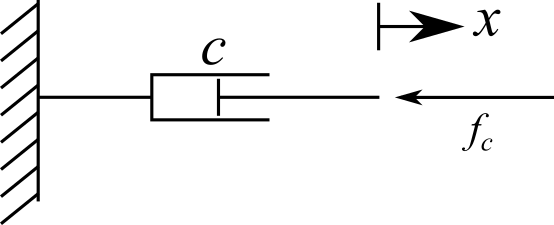
\includegraphics[]{../figures/linear_dashpot.png}
			\caption{Schematic of a liner dashpot showing the damping force ($f_c$) acting in the opposite direction of the displacement ($x$).}
			\label{fig:linear_dashpot}
		\end{figure}
		
		Just as spring forms a physical model of the cause vibration, through its storage and release of energy, a dashpot (sometimes called a damper) forms a physical model for dissipating energy. Dashpots create a resisting or damping force that acts opposite to the direction of travel (as annotated in figure \ref{fig:linear_dashpot}) and is proportional to the velocity. Therefore, the damping forces $f_c$ can be computed as:
		\begin{equation}
			f_c = c \dot{x}
		\end{equation}
		the constant $c$, called the damping coefficient, has the units of kg/s. Dashpots are a mathematical representation of viscous dampers installed in automobiles, aircraft, structures, and other mechanical devices. However, all systems have inherent damping not just systems with physical dampers. The spring-mass system can be used as a representations of real-world systems with inherent damping as demonstrated by the rubber engine mount depicted in figure \ref{fig:rubber_engine_mount}.
		
		
		\begin{figure}[H]
			\centering
			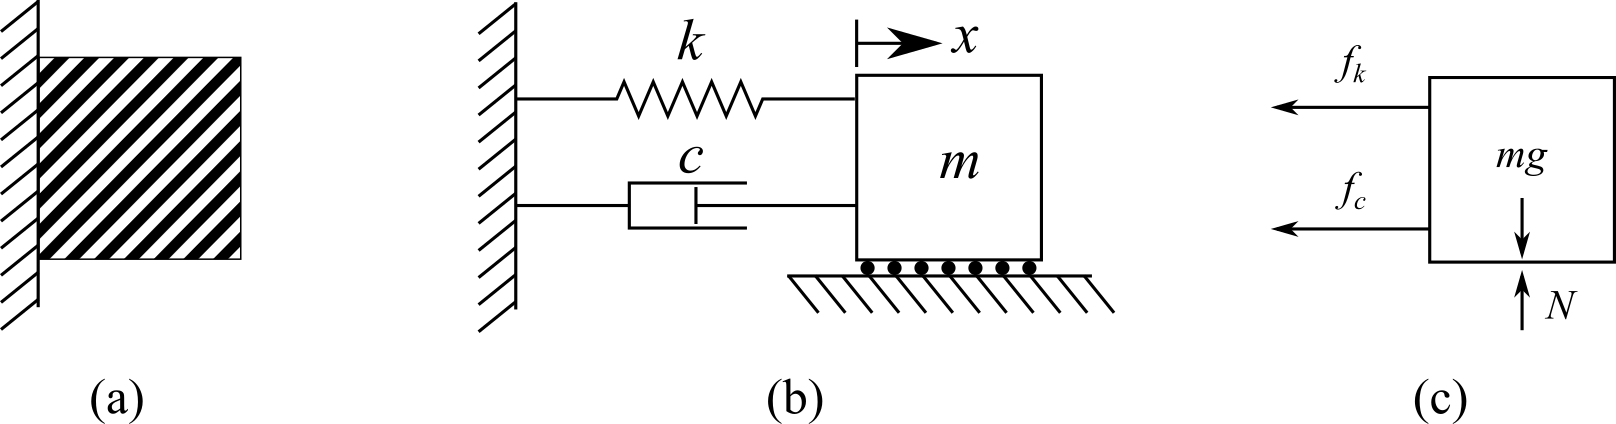
\includegraphics[]{../figures/engine_mount_model.png}
			\caption{Modeling of a rubber engine mount as an spring-dashpot-mass model showing (a) the rubber engine mount; (b) idealized model of the rubber month; and (c) the FBD of the idealized model}
			\label{fig:rubber_engine_mount}
		\end{figure}

		Depending on the amount of damping present in a system, the temporal response of the system will represent itself in various way, as represented in figure \ref{fig:damping_cases}. To reiterate, an undamped case will oscillates around the equilibrium and does not decay. If a limited amount of damping is present in a system it will oscillates around the equilibrium and slowly decay with time to the equilibrium position, this is termed underdamped. If an excessive amount of damping is present, the system will not oscillate but decay directly to the equilibrium position, this is termed the overdamped case. Lastly, there exists a special case that results in the system converging as quickly as possible to the equilibrium position without oscillations; this cases is termed the critically damped case. Furthermore, the amount of damping required to obtain a critically damped system is the damping value that the underdamped and overdamped cases for a specific system. To recap, the key types of damping are:
		
		\begin{itemize}
			\item \textbf{Undamped} - Oscillates around the equilibrium and does not decay.
			\item \textbf{Underdamped} - Oscillates around the equilibrium and slowly decays  and is the most common case.
			\item \textbf{Overdamped} - Does not pass the equilibrium position and is a simple a decay with no oscillation.
			\item \textbf{Critically damped} - provides the quickest approach to zero amplitude for a damped oscillator.
		\end{itemize}
		
		
		\begin{figure}[H]
			\centering
			\includegraphics[]{../figures/damping_cases.png}
			\caption{Temporal responses for the three types of damping: underdamped, over damped, and critically damped.}
			\label{fig:damping_cases}
		\end{figure}
			
		\subsubsection{Modeling Vibrating Systems with Damping}
				
			The spring-mass system of chapter 1 can be expanded to a spring-dashpot-mass system that considers the damping component of the system. A mathematical model of the 	spring-dashpot-mass system can be developed for the case present in figure \ref{fig:1-DOF-mass_horizontal_damping_FBD}. Using the FBD for the system, it can conclude that the EOM for this system:
			\begin{figure}[H]
				\centering
				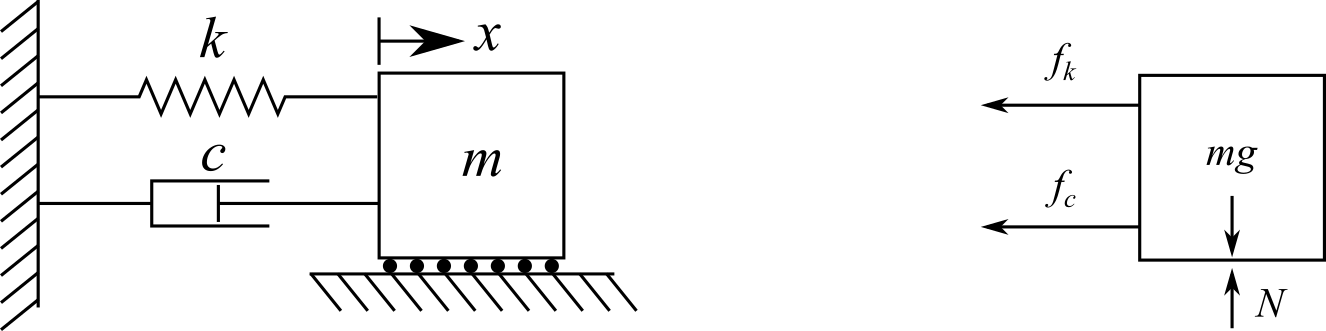
\includegraphics[]{../figures/1_DOF_spring_dashpot_mass_horizontal_FBD.png}
				\caption{Spring-dashpot-mass model showing: (a) a schematic of the system; and (b) the FBD of the system. }
				\label{fig:1-DOF-mass_horizontal_damping_FBD}
			\end{figure}			
			\noindent is:
			\begin{equation}
				m\ddot{x}(t) = - f_c - f_k
			\end{equation}
			Rearranging into standard form and concerting forces into parameters $c$ and $k$ results in:
			\begin{equation}
				m\ddot{x}(t) + c \dot{x}(t) + kx(t) = 0
			\end{equation}
			This system is subject to the same initial conditions as before, $x(0) = x_0$ and $\dot{x}(0) = v_0$. Again, choosing to model it this way for convinces, so let's solve it in a similar manner to the EOM without damping. Again, assume the solution:
			\begin{equation}
				x(t) = ae^{\lambda t}
			\end{equation}
			here, $a$ and $t$ are nonzeros constants that need to be determined.  Using successive differentiation, we get:
			\begin{equation}
				\dot{x}(t) = \lambda ae^{\lambda t}
			\end{equation}
			and 
			\begin{equation}
				\ddot{x}(t) = \lambda^2 ae^{\lambda t}
			\end{equation}
			therefore, $m\ddot{x} + c\dot{x} + kx = 0$ becomes:
			\begin{equation}
				m \lambda^2 ae^{\lambda t}  +c\lambda ae^{\lambda t} + k ae^{\lambda t} = 0
			\end{equation}
			Now we divide by $ae^{\lambda t}$ to obtain the \textbf{characteristic equation}:
			\begin{equation}
				m \lambda^2 + c\lambda + k = 0
			\end{equation}
			We can do this because $ae^{\lambda t}$ is never zero, therefore, we never divide by zero. The quadratic formula gives us:
			\begin{equation}
				\lambda_{1,2} = \frac{-c \pm \sqrt{c^2-4km}}{2m}  = \frac{-c}{2m} \pm \frac{1}{2m}\sqrt{c^2-4km}
			\end{equation}
			Some key points from this equation:
			\begin{itemize}
			\item The $\pm$ tells us there are two solutions to this problem
			\item if $c^2-4km<0$, system is Underdamped, solutions are complex conjugate pairs 
			\item if $c^2-4km=0$, system is critically damped, solutions are equal negative real numbers 
			\item if $c^2-4km>0$, system is Overdamped, solutions are distinct negative real numbers 
			\end{itemize}
			From this, we can see that $c^2-4km=0$ is a special value, let us define a value for $c$ that will give us this critical damping number. We will call it the \textbf{critical damping coefficient} ($c_{\text{cr}}$). So setting the equation as:
			\begin{equation}
				c_{\text{cr}}^2-4km = 0
			\end{equation}
			giving us: 
			\begin{equation}
				c_{\text{cr}}^2 = 4km
			\end{equation}		
			next we can derive the function:
			\begin{equation}
				c_{\text{cr}} = 2\sqrt{km} = 2\bigg(\frac{\sqrt{m}}{\sqrt{m}}\bigg)\sqrt{km} = 2m\omega_n
			\end{equation}			
			remember that $\omega_n = \sqrt{\frac{k}{m}}$ for an undamped system. Next, we generate a non-dimensional number ($\zeta$), pounced `zeta' that will allow us to distinguish between different types of damping. $\zeta$ is called the \textbf{critical damping ratio}.
			\begin{equation}
				\zeta = \frac{c}{c_{\text{cr}}} = \frac{c}{2\sqrt{km}} = \frac{c}{2m\omega_n}
			\end{equation}				
			Now if we put the $\zeta$ back into the characteristic equation and resolve using the quadratic equation we get: 
			\begin{equation}
				\lambda_{1,2} = -\zeta\omega_n \pm \omega_n \sqrt{\zeta^2-1}
			\end{equation}
			From this equation it become clear that $\zeta$ determines whether the roots are complex or real, this in turn determines the nature of the response of the structure. Listing our possible responses we get:
			\begin{table}[h!]
				\centering
				\begin{tabular}{lccc}
					\toprule
					damping case & critical damping ratio & radicand & solutions  \\ \midrule
					under damped &  $0<\zeta<1$ & $c^2-4km<0$ & complex conjugate pairs \\
					critically damped & $\zeta=1$ & $c^2-4km=0$ & equal negative real numbers \\
					over damped & $1<\zeta$  & $c^2-4km>0$ & distinct negative real numbers \\ \bottomrule
				\end{tabular}
			\end{table}
			For each damping case, we will have a different solution to the problem. 
					
		\subsubsection{Modeling Underdamped Motion}
		
 			In the case that $0<\zeta<1$, a complex conjugate pair of roots are the solutions to the characteristic equation after pulling out a $\sqrt{-1}$:
			\begin{equation}
				\lambda_{1} = -\zeta\omega_n + \omega_n \sqrt{1-\zeta^2}j
			\end{equation} 			
			and:
			\begin{equation}
				\lambda_{2} = -\zeta\omega_n - \omega_n \sqrt{1-\zeta^2}j
			\end{equation} 
			Where the $j$ is pulled out because:
			\begin{equation}
				\sqrt{1-\zeta^2}j = \sqrt{(1-\zeta^2)(-1)} = \sqrt{\zeta^2-1}
			\end{equation} 							
			Next, let us ``arbitrarily'' define:
			\begin{equation}
				\omega_d = \omega_n\sqrt{1-\zeta^2}
			\end{equation} 	
			where $\omega_d$ is the \textbf{damped natural frequency}. Therefore, the equations become:
			\begin{equation}
				\lambda_{1} = -\zeta\omega_n + \omega_dj
			\end{equation} 			
			and:
			\begin{equation}
				\lambda_{2} = -\zeta\omega_n - \omega_dj
			\end{equation} 	
			Again, we have two solutions to a linear problem, so we can combine these into one solution and insert $\lambda$ into the assumed solution $ae^{\lambda t}$ to obtain:
			\begin{equation}
				x(t) = a_1e^{-\zeta\omega_nt + \omega_dtj} + a_2e^{-\zeta\omega_nt - \omega_dtj} 
			\end{equation} 			
			where $a_1$ and $a_2$ are complex valued constants. This can now be simplified into:	
			\begin{equation}
				x(t) = e^{-\zeta\omega_nt}(a_1e^{\omega_dtj} + a_2e^{-\omega_dtj}) 
			\end{equation} 
			Using Euler's equations, (same as before) and choosing:
			\begin{equation}
				A_1=(a_1-a_2)j
			\end{equation} 	
			and
			\begin{equation}
				A_2=(a_1+a_2)
			\end{equation} 		
			The \textbf{general form} of this solution is then:
			\begin{equation}
				x(t) = e^{-\zeta\omega_nt}\big(A_1\text{sin}(\omega_dt) + A_2\text{cos}(\omega_dt)\big)
			\end{equation} 	
			Recall that for undamped 1-DOF systems we showed 
			\begin{equation}
				x(t) = A\text{sin}(\omega_nt + \phi) = A_1\text{sin}(\omega_nt) + A_2\text{cos}(\omega_nt)
			\end{equation} 				
			As $e^{-\zeta\omega_nt}$ accounts for the damping, our current solution becomes:
			\begin{equation}
				x(t) = Ae^{-\zeta\omega_nt}\text{sin}(\omega_dt + \phi) 
			\end{equation} 		
			Now that we have $x$ and $\dot{x}$, we can solve for the boundary conditions $x_0$ and $v_0$ by setting $t=0$, we get:
			\begin{equation}
				x(0)=x_0 = A\text{sin}(\phi) 
			\end{equation} 			
			and taking the directive of $x(t)$ using the product rule (fg)'= f'g+fg', we get:
			\begin{equation}
				\dot{x}(t) = -\zeta\omega_nAe^{-\zeta\omega_nt}\text{sin}(\omega_dt + \phi) + Ae^{-\zeta\omega_nt}\omega_d\text{cos}(\omega_dt + \phi) 
			\end{equation} 
			\begin{equation}
				\dot{x}(0) =v_0= -\zeta\omega_nA\text{sin}(\phi) + A\omega_d\text{cos}(\phi) 
			\end{equation} 
			a simplification can be made to the prior equation by letting $A=x_0/\text{sin}(\phi)$. This gives us the equation:
			\begin{equation}
				\dot{x}(0) =v_0= -\zeta\omega_n\bigg(\frac{x_0}{\text{sin}(\phi)}\bigg)\text{sin}(\phi) + \bigg(\frac{x_0}{\text{sin}(\phi)}\bigg)\omega_d\text{cos}(\phi) 
			\end{equation} 			
			that can be simplified to:
			\begin{equation}
				\dot{x}(0) = v_0 = -\zeta\omega_nx_0 + x_0\omega_d\text{cot}(\phi) 
			\end{equation} 	
			The above equation related $v_0$ to $\phi$ using terms that are known for a giving system ($\zeta,\, \omega_n,\, x_0 \text{, and }\omega_d $). Therefore, this expression can be used to solve for $\phi$:
			\begin{equation}
				\text{cot}(\phi) = \frac{v_0 +\zeta\omega_nx_0}{x_0\omega_d} 
				\label{eq:underdamped_phi}
			\end{equation} 	
			and as the $\text{tan}(\phi) = 1/\text{cot}(\phi)$: 
			\begin{equation}
				\phi = \text{tan}^-1\Bigg(\frac{x_0\omega_d}{v_0+\zeta\omega_nx_0}\Bigg)
			\end{equation} 				
			Thereafter, we can solve for $A$ considering the fact that we sent $A=x_0/\text{sin}(\phi)$. Using the trigonometric relationship between expressed in equation \ref{eq:underdamped_phi} and visualized in figure \ref{fig:trigonometric_relationship_underdamped}:
			\begin{figure}[H]
				\centering
				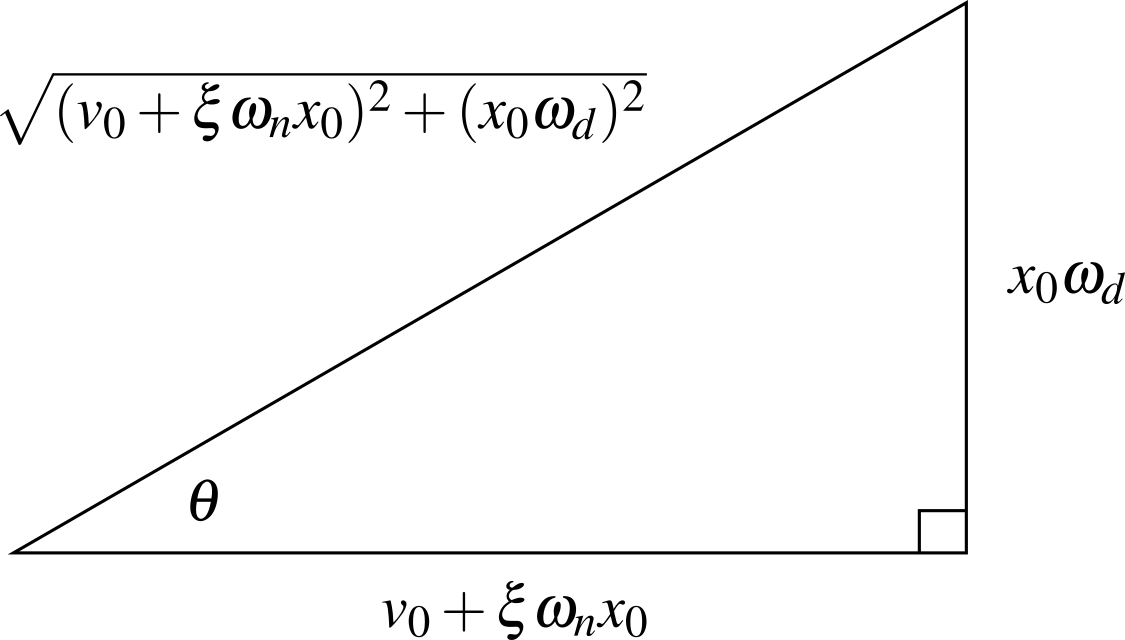
\includegraphics[]{../figures/Trigonometric_relationship_underdamped.png}
				\caption{Trigonometric relationship between the initial conditions ($x_0$ and $v_0$), amplitude $A$, and phase $\phi$ for underdamped motion of a 1-DOF system.}
				\label{fig:trigonometric_relationship_underdamped}
			\end{figure}
			\noindent we show that $\text{sin}(\phi)$ can be expressed as: 
			\begin{equation}
				\text{sin}(\phi) = \frac{x_0\omega_d}{\sqrt{(v_0+\zeta\omega_nx_0)^2 + (x_0\omega_d)^2}}
			\end{equation} 	
			and applying $A=x_0/\text{sin}(\phi)$ we get:
			\begin{equation}
				A = \frac{\sqrt{(v_0+\zeta\omega_nx_0)^2 + (x_0\omega_d)^2}}{\omega_d} = \sqrt{x_0^2 + \Bigg( \frac{v_0 + \zeta \omega_n x_0}{\omega_d}\Bigg)^2}
			\end{equation} 								
			Finally, collecting all of our important equations:
			\begin{itemize}
			\item Critical damping coefficient: $c_{\text{cr}} = 2\sqrt{km} = 2m\omega_n$
			\item Damping ratio: $	\zeta = \frac{c}{c_{\text{cr}}} = \frac{c}{2\sqrt{km}} = \frac{c}{2m\omega_n}$
			\item Damped natural frequency: $\omega_d = \omega_n\sqrt{1-\zeta^2}$
			\item Solution for underdamped system: $x(t) = Ae^{-\zeta\omega_nt}\text{sin}(\omega_dt + \phi)$, where: \begin{align*}
						A = \frac{\sqrt{(v_0+\zeta\omega_nx_0)^2 + (x_0\omega_d)^2}}{\omega_d} & \hspace{1.5cm} \phi = \text{tan}^-1\Bigg(\frac{x_0\omega_d}{v_0+\zeta\omega_nx_0}\Bigg) 
						\end{align*}
			\end{itemize}

			\begin{figure}[H]
				\centering
				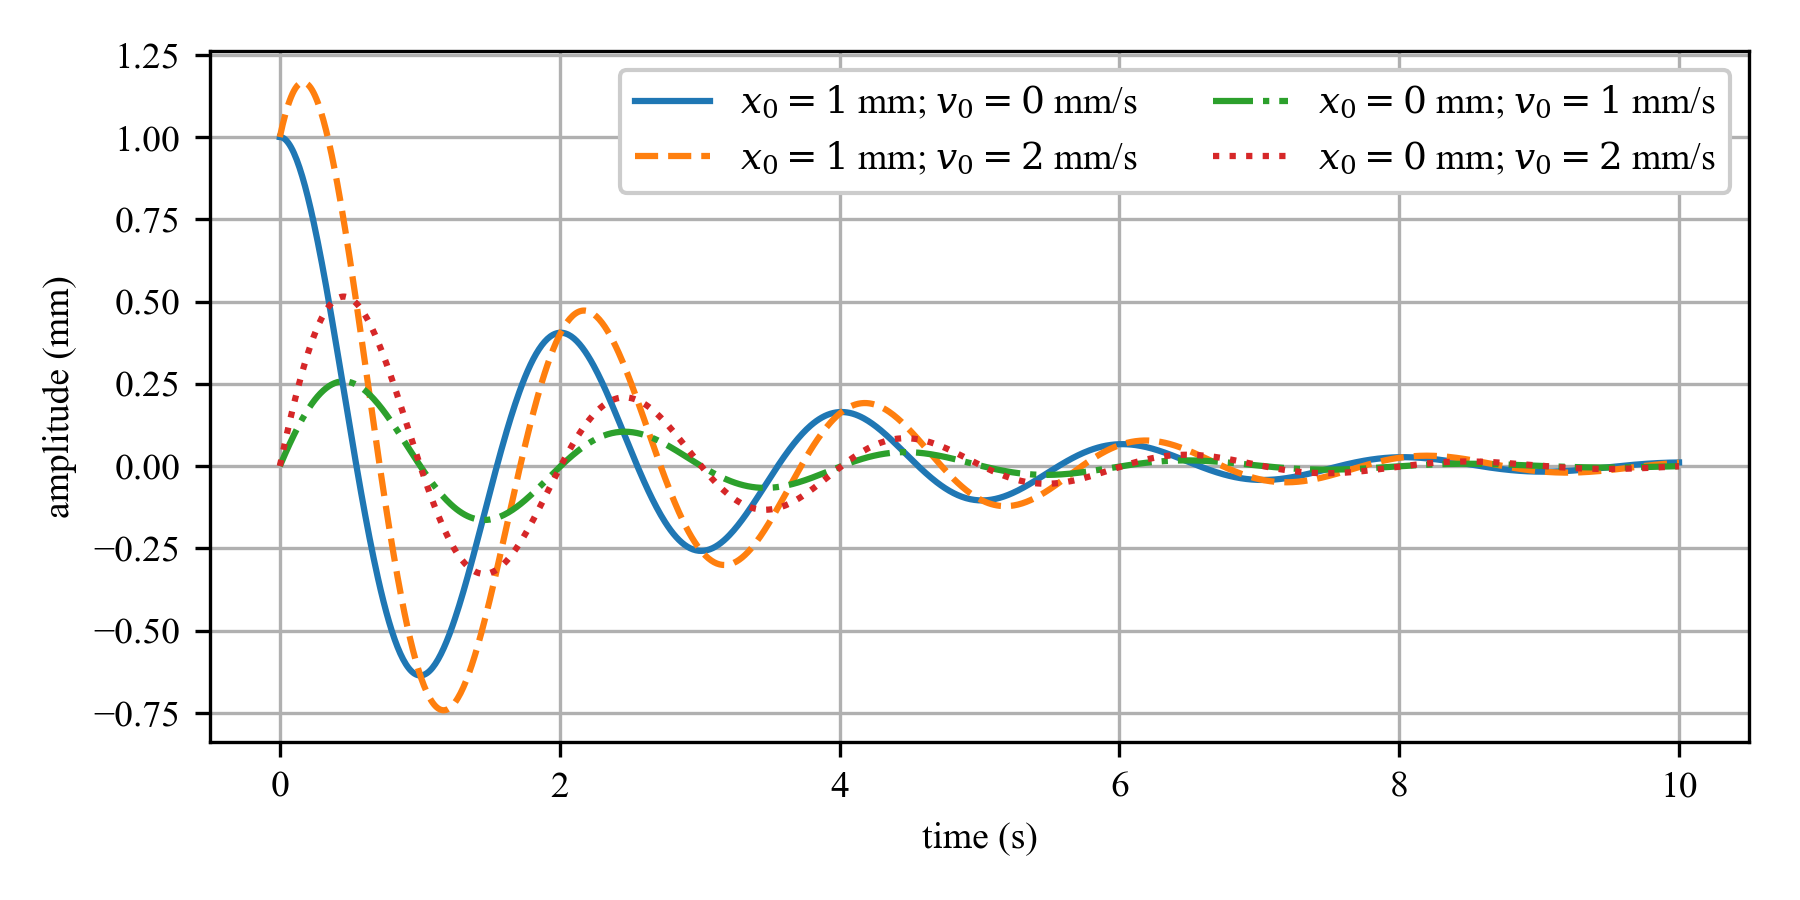
\includegraphics[]{../figures/Under_damped_various_initial_conditions.png}
				\caption{Four example responses for an under damped 1-DOF system  ($\zeta=0.142$) with various initial conditions.}
			\end{figure}

		\begin{example}				
			Consider the following 1-DOF system, where $k = 857.8$ N/m, $c=7.8$ kg/s, and $m=49.2\times10^{-3}$ kg, calculate the damped frequency in rad/s and Hz. What damping case is this system?  
			\begin{figure}[H]
				\centering
				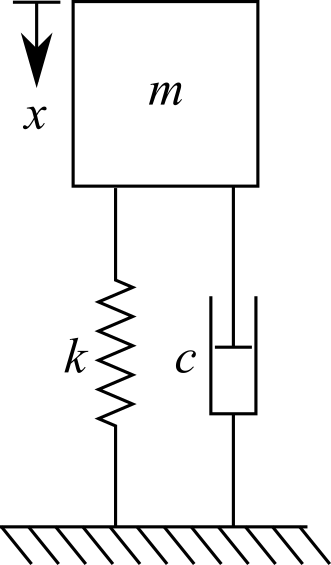
\includegraphics[]{../figures/1_DOF_spring_dashpot_mass_vertical.png}
				\caption{1-DOF spring-dashpot-mass system.}
			\end{figure}		

			\noindent\textbf{Solution:} 
			
			Calculate the undamped frequency:
			\begin{equation}
				\omega_n = \sqrt{\frac{k}{m}}= \sqrt{\frac{857.8}{49.2\times10^{-3}}} = 132 \hspace{1ex}\text{rad/s}
			\end{equation}	
			The systems critical damping value:
			\begin{equation}
				c_{\text{cr}} = 2\sqrt{km}= 2\sqrt{k = 857.8 \cdot 49.2\times10^{-3}} = 12.993 \hspace{1ex}\text{kg/s}
			\end{equation}		
			And the critical damping ratio:
			\begin{equation}
				\zeta = \frac{c}{c_{\text{cr}}} = \frac{7.8}{12.993} = 0.600
			\end{equation}				
			This can also be expressed as 60\% damped, this is a underdamped system, and the system will oscillate. Now we can calculate the damped frequency:
			\begin{equation}
				\omega_d = \omega_n\sqrt{1-\zeta^2} = \omega_n\sqrt{1-0.600^2} = 105.6 \hspace{1ex}\text{rad/s}
			\end{equation}		
			Therefore, the system oscillates at 105.6 rad/sec or 16.81 Hz
		\end{example}

		\begin{example}
			For a damped one DOF system where $m$, $c$, and $k$ are known to be $m$ = 1 kg, $c$ = 2 kg/s, and $k$ = 10 N/m. Calculate the value of $\zeta$ and $\omega_n$. Is the system overdamped, underdamped, or critically damped?	

			\noindent\textbf{Solution:} 
						
			The natural frequency is calculated as
			\begin{equation}
				\omega_n = \sqrt{\frac{k}{m}} = \sqrt{\frac{10}{1}} = 3.16 \hspace{1ex} \text{rad/s}
			\end{equation}
			The damping can be calculated as:
			\begin{equation}
				\zeta = \frac{c}{2\omega_n m} = \frac{2}{2\Big(\sqrt{\frac{10}{1}}\Big)(1)} = \frac{1}{\sqrt{10}} = 0.316 
			\end{equation}
			So the damped natural frequency is equal to:
			\begin{equation}
				\omega_d = \omega_n\sqrt{1-\zeta^2} =  \sqrt{10}\sqrt{1-\bigg(\frac{1}{\sqrt{10}}\bigg)^2} = 0.3 \hspace{1ex} \text{rad/s}
			\end{equation}			
			As $0<\zeta<1$ the system is underdamped. 			
		\end{example}

		\begin{example}
			For the following industrial device consisting of a mass isolated from its fixtures by two rubber dampers and a offset spring provide an estimate of the system's damped natural frequency in the vertical direction.	Assume the the rubber dampers add damping and only negligible stiffness to the system and that the spring is long enough such that the angles remain constant. 	
			\begin{figure}[H]
				\centering
				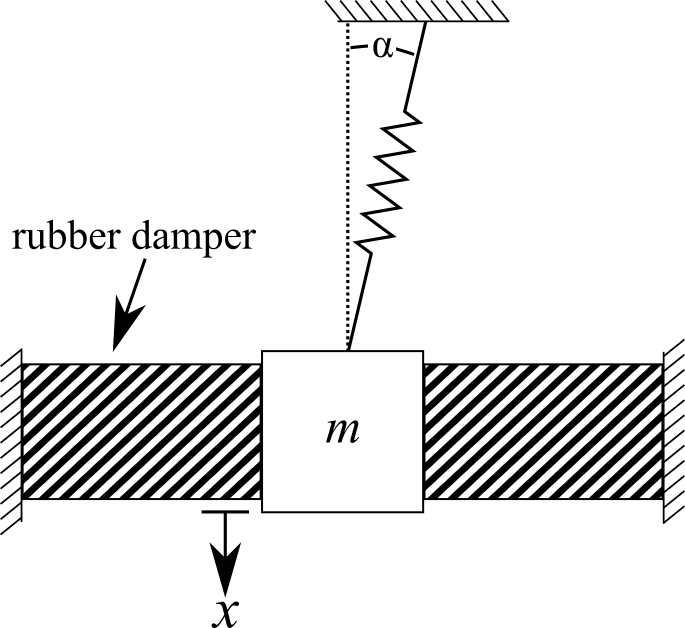
\includegraphics[]{../figures/rubber_mounted_mass_with_spring.png}
				\caption{Industrial device (mass) connected to a fixed point with a rubber damper and spring at an angle.}
				\label{fig:rubber_mounted_mass_with_spring}
			\end{figure}
	
			\noindent\textbf{Solution:} 
			
			First and foremost, we need to develop a mass-spring-dashpot representation of the system. The is presented in what follows:
			
			\begin{figure}[H]
				\centering
				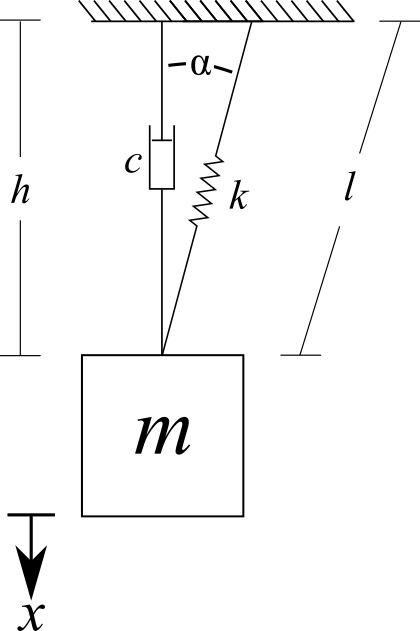
\includegraphics[]{../figures/rubber_mounted_mass_with_spring_spring_dashpot_system.png}
				\caption{Mass-spring-dashpot representation of the industrial system represented if figure \ref{fig:rubber_mounted_mass_with_spring}.}
			\end{figure}
				
			where the damping in the vertical direction provided by the rubber damper is modeled a dashpot in the vertical direction. As we only want an estimate of the frequency, the assumption that the is small and as such $\alpha$ of the displaced state is equal $\alpha$ of the equilibrium state. This leads to the FBD for the equilibrium  and displaced states:
			
			\begin{center}
				equilibrium position \hspace{4cm} displaced position ``x''
			\end{center}
			\begin{figure}[H]
				\centering
				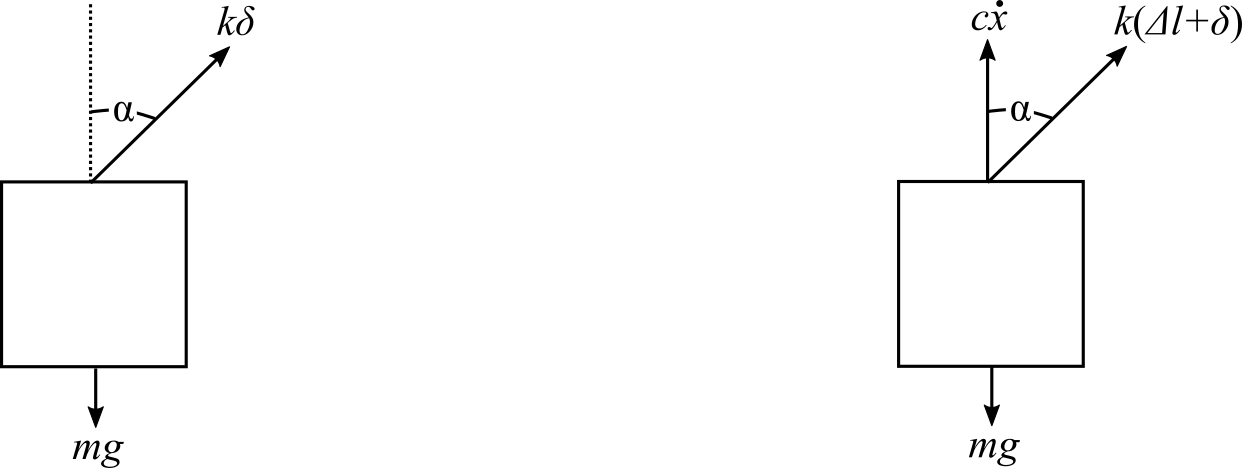
\includegraphics[]{../figures/rubber_mounted_mass_with_spring_FBD.png}
			\end{figure}
			The equation for the equilibrium state is:
			\begin{equation*}
				\downplus \sum F_x = mg -k\delta\text{cos}(\alpha) =0
			\end{equation*}
			and in the displaced state:
			\begin{equation*}
				\downplus \sum F_x = mg - c\dot{x}-k\text{cos}(\alpha)(\Delta l+\delta)
			\end{equation*}
			Applying Newton's second law and combining these equations yields:
			\begin{equation*}
				m\ddot{x} + c\dot{x} + k \Delta l \text{cos}(\alpha) =0
			\end{equation*}	
			Looking at the triangles formed by the dashpot and spring it can be shown that:
			\begin{equation*}
				 \cos(\alpha) = h/l = x/\Delta l  
			\end{equation*}			
			As we assumed the displacement is small and $\alpha$ remains unchanged. Therefore the prior equation becomes: 
			\begin{equation*}
				m\ddot{x} + c\dot{x} + k \Delta l \frac{x}{\Delta l} = 0
			\end{equation*}	
			This simplifies to the ``normal'' EOM for a 1-DOF system: 
			\begin{equation*}
				m\ddot{x} + c\dot{x} + k x  = 0
			\end{equation*}				
			Therefore, once the values for the system are measured the system's damped natural frequency in the vertical direction can be estimated as		
			\begin{equation*}
				\boxed{\omega_d = \omega_n\sqrt{1-\zeta^2}}
			\end{equation*}
		\end{example}	
				
		\subsubsection{Modeling Overdamped Motion}
			
			In the case of overdamped systems, $1<\zeta$, the solutions for $\lambda$ are distinct real roots that are written as:
			\begin{equation}
				\lambda_{1} = -\zeta\omega_n - \omega_n \sqrt{\zeta^2-1}
			\end{equation} 			
			and:
			\begin{equation}
				\lambda_{2} = -\zeta\omega_n + \omega_n \sqrt{\zeta^2-1}
			\end{equation} 
			The solution for the EOM using the assumed solution then becomes:
			\begin{equation}
				x(t) = e^{-\zeta\omega_nt}(a_1e^{-\omega_n t \sqrt{\zeta^2-1}} + a_2e^{+\omega_n t \sqrt{\zeta^2-1}}) 
			\end{equation}
			This equation represents a non-oscillating response of the system. Again, $a_1$ and $a_2$ are solved for using known boundary conditions $x_0$ and $v_0$ such that:
			\begin{align}
				a_1 &= \frac{-v_0+\Big(-\zeta+\sqrt{\zeta^2-1}\Big)\omega_n x_0}{2\omega_n\sqrt{\zeta^2-1}} \\ 
				a_2 &= \frac{v_0+\Big(\zeta+\sqrt{\zeta^2-1}\Big)\omega_n x_0}{2\omega_n\sqrt{\zeta^2-1}}
			\end{align}				
			Typical responses for a overdamped system with various initial conditions are shown below:
			\begin{figure}[H]
				\centering
				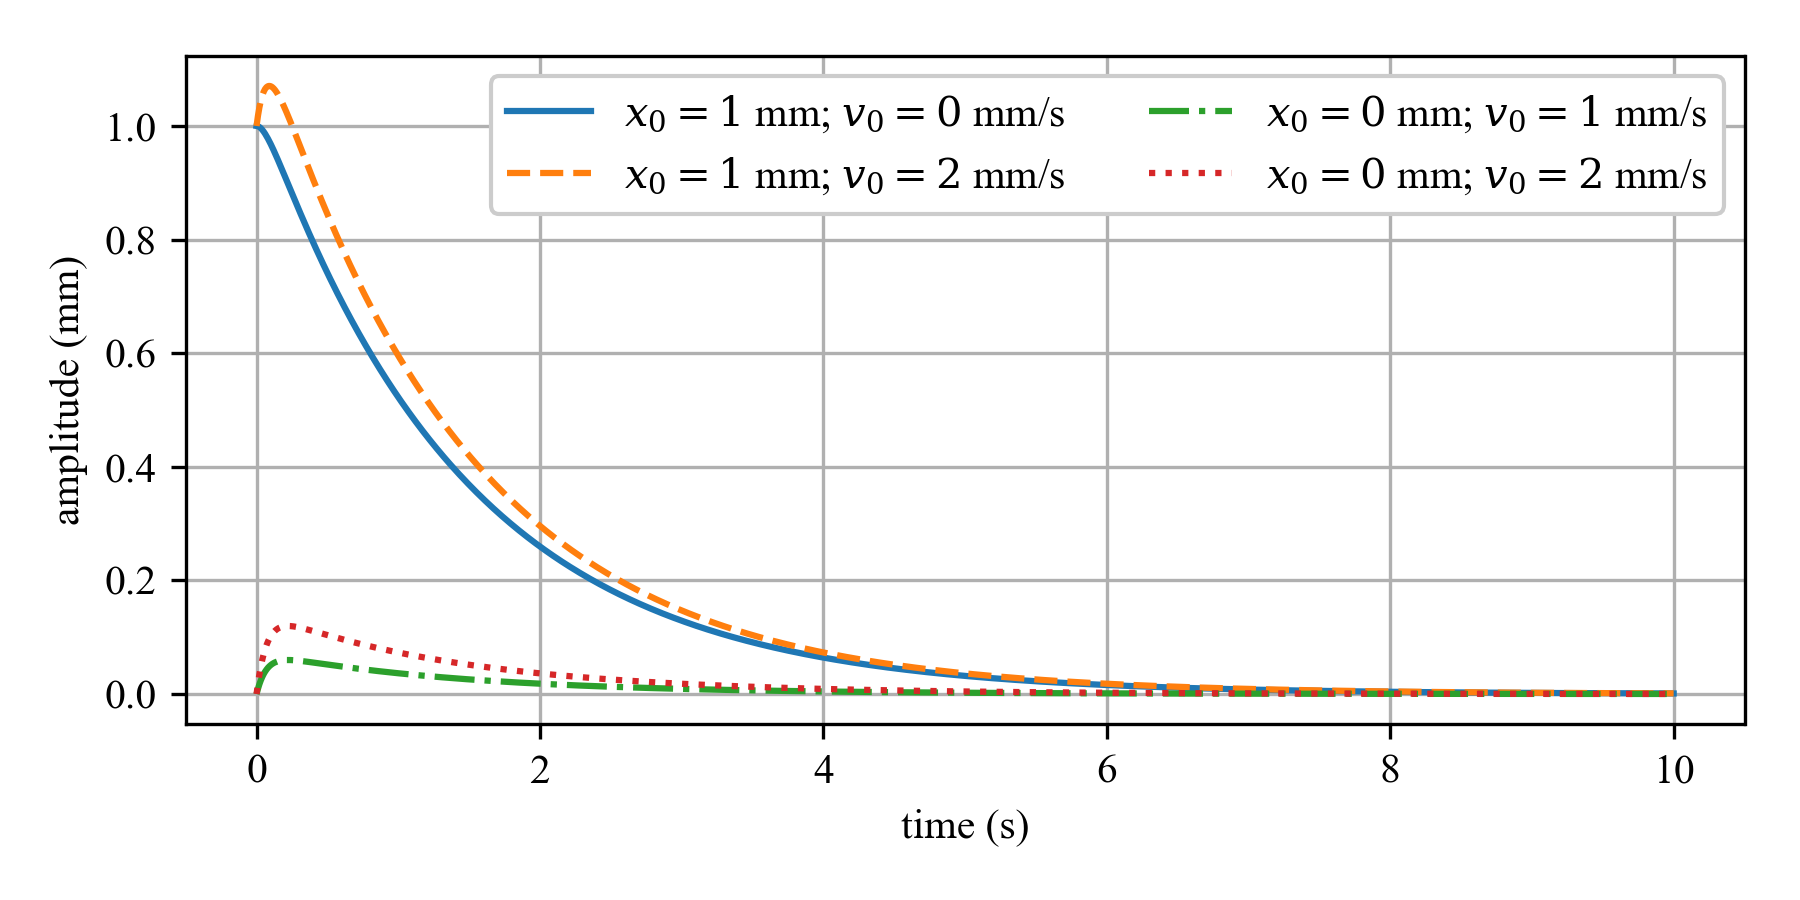
\includegraphics[]{../figures/Over_damped_various_initial_conditions.png}
				\caption{Four example responses for an over damped 1-DOF system ($\zeta=2.371$) with various initial conditions.}
			\end{figure}

		\subsubsection{Modeling critically damped motion}			

			In the case of critically damped systems, $\zeta=1$, the solutions for $\lambda$ will be equal negative real numbers, therefore from before:
			\begin{equation}
				\lambda_{1,2} = -\zeta\omega_n \pm \omega_n \sqrt{\zeta^2-1}
			\end{equation}
			We get:
			\begin{equation}
				\lambda_{1} = \lambda_{2} = -\omega_n
			\end{equation} 			
			Because both solutions ($a_1$ and $a_2$) are the same, we multiply the second solution by $t$ so the solution for a critically damped system is in the same form as before. The solution for the EOM using the assumed solution then becomes:
			\begin{equation}
				x(t) = a_1e^{-\omega_nt} + a_2te^{-\omega_nt} 
			\end{equation} 
			This simplifies into:			
			\begin{equation}
				x(t) = (a_1+a_2t) e^{-\omega_nt} 
			\end{equation}
			This equation represents a non-oscillating response of the system. Again, $a_1$ and $a_2$ are solved for using known boundary conditions $x_0$ and $v_0$ such that:
			\begin{align}
				a_1 &= x_0 \\ 
				a_2 &= v_0+\omega_nx_0
			\end{align}				


		\subsubsection{Standard Form of the EOM}
			
			The EOM for a damped 1-DOF system is written in a ``standard form'' in which the effect of the damping ration and natural frequencies are more obvious. To get to the standard form, the normal form of the EOM:
			\begin{equation}
				m\ddot{x} + c \dot{x} + kx = 0
			\end{equation}
			is divided by what the constant terms associated with the acceleration term. In this example, this is $m$. Dividing every term by $m$ yields: 
			\begin{equation}
				\ddot{x} + \frac{c}{m}\dot{x} + \frac{k}{m}x = 0
			\end{equation}		
			Numerical manipulations can be undertaken to get the coefficients of the velocity and displacement terms into coefficients that more clearly express the characteristics of the vibrating system:
			\begin{equation}
				\ddot{x} + 2\zeta\omega_n\dot{x} + \omega_n^2x = 0
			\end{equation}	

		\begin{example}

		A engine valve assembly depicted is figure \ref{fig:engine_valve} where $J$ is the inertia caused by the right-hand side of the rocker arm. Derive an analytical solution for the natural frequency of the rocker arm. Use the assumptions sin($\theta$) = $\theta$ and cos($\theta$) = 1.
		
			\begin{figure}[H]
				\centering
				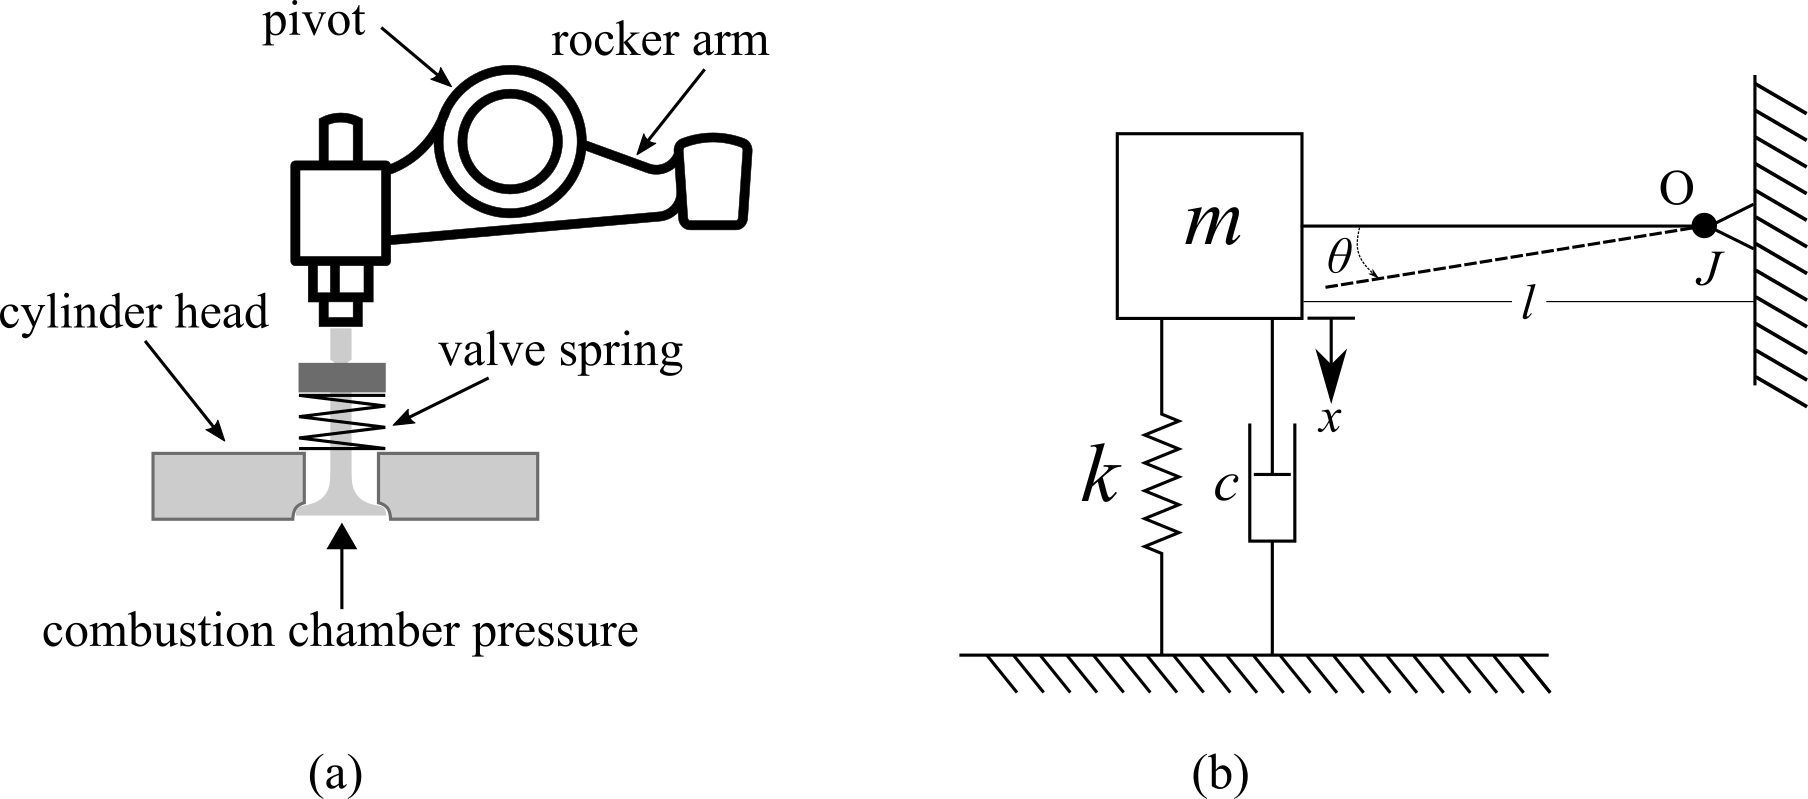
\includegraphics[]{../figures/engine_valve.png}
				\caption{Rocker arm assembly of an internal combustion engine showing: (a) a diagram of the system and; (b) the FBD of the system.}
				\label{fig:engine_valve}
			\end{figure}
			
		\noindent\textbf{Solution:} 
		
		Taking the sum of the moments about $O$ and considering the inertia caused by the right-hand side of the rocker arm, $J$, the FBDs can be written as: 
		\begin{center}
			equilibrium position \hspace{4cm} displaced position ``x''
		\end{center}
		\begin{figure}[H]
			\centering
			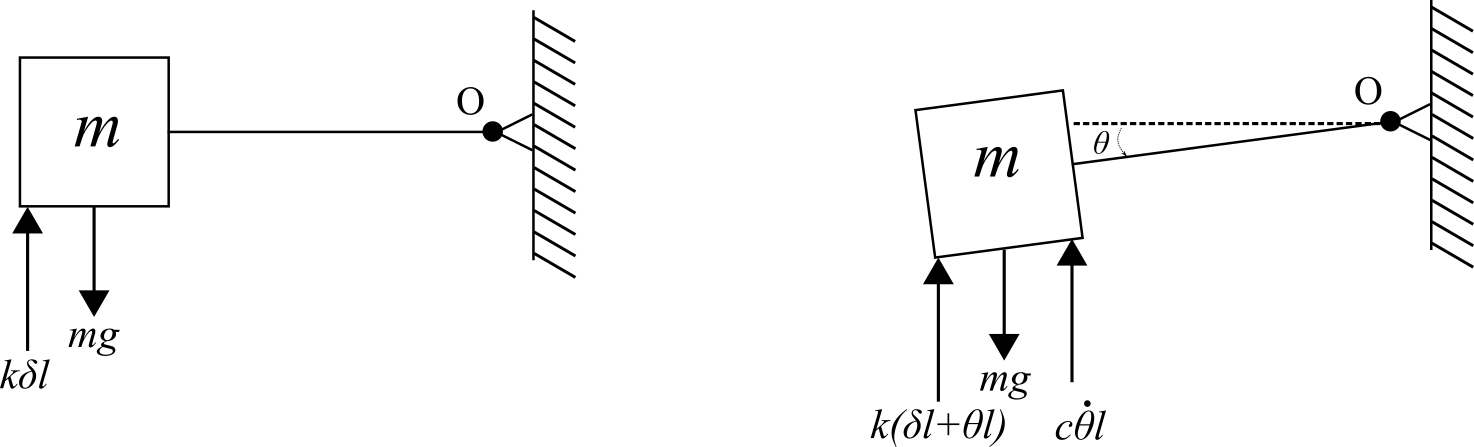
\includegraphics[]{../figures/engine_valve_FBD.png}
		\end{figure}
		The equation for the equilibrium state is:
		\begin{equation*}
			\curveplus \sum M_o = mgl -k l^2 \delta =0
		\end{equation*}
		and in the displaced state:
		\begin{equation*}
			\curveplus \sum M_o = mgl -k l^2 \delta -k l^2 \theta -c l^2\dot{\theta} =0
		\end{equation*}
		Applying Newton's second law and combining these equations yields:
		\begin{equation}
			(J+ml^2)\ddot{\theta} +cl^2\dot{\theta} + kl^2 \theta = 0
		\end{equation}	
		Therefore, the standard form of the EOM is:
		\begin{equation}
			\ddot{\theta} + \frac{cl^2}{J+ml^2}\dot{\theta} + \frac{kl^2 }{J+ml^2}\theta  = 0
		\end{equation}	
		Results in the following analytical solution for the natural frequency:
		\begin{equation}
			\omega_n = \sqrt{\frac{kl^2 }{J+ml^2}} \text{ rad/s}
		\end{equation}	
							
		\end{example}	

	

		\subsection{Logarithmic decrement}
			
			For a vibrating system, the  mass ($m$) and stiffness ($k$) can be measured using scales and static deflection tests. However, the damping coefficient ($c$) is a more difficult quantity to determine. From $k$ and $m$ we can compute the natural frequency ($\omega_n$) and the critical damping coefficient ($c_\text{cr}$). Therefore, knowing that the critical damping ratio ($\zeta$) is defined as:
			\begin{equation}
				\zeta = \frac{c}{c_{\text{cr}}} = \frac{c}{2\sqrt{km}} = \frac{c}{2m\omega_n}
			\end{equation}				
			if we calculate $\zeta$, we can obtain $c$ for the system of interest. This is made possible because $c_\text{cr}$ can be calculated from $k$ and $m$. Observing the temporal response for the underdamped system, 
			\begin{figure}[H]
				\centering
				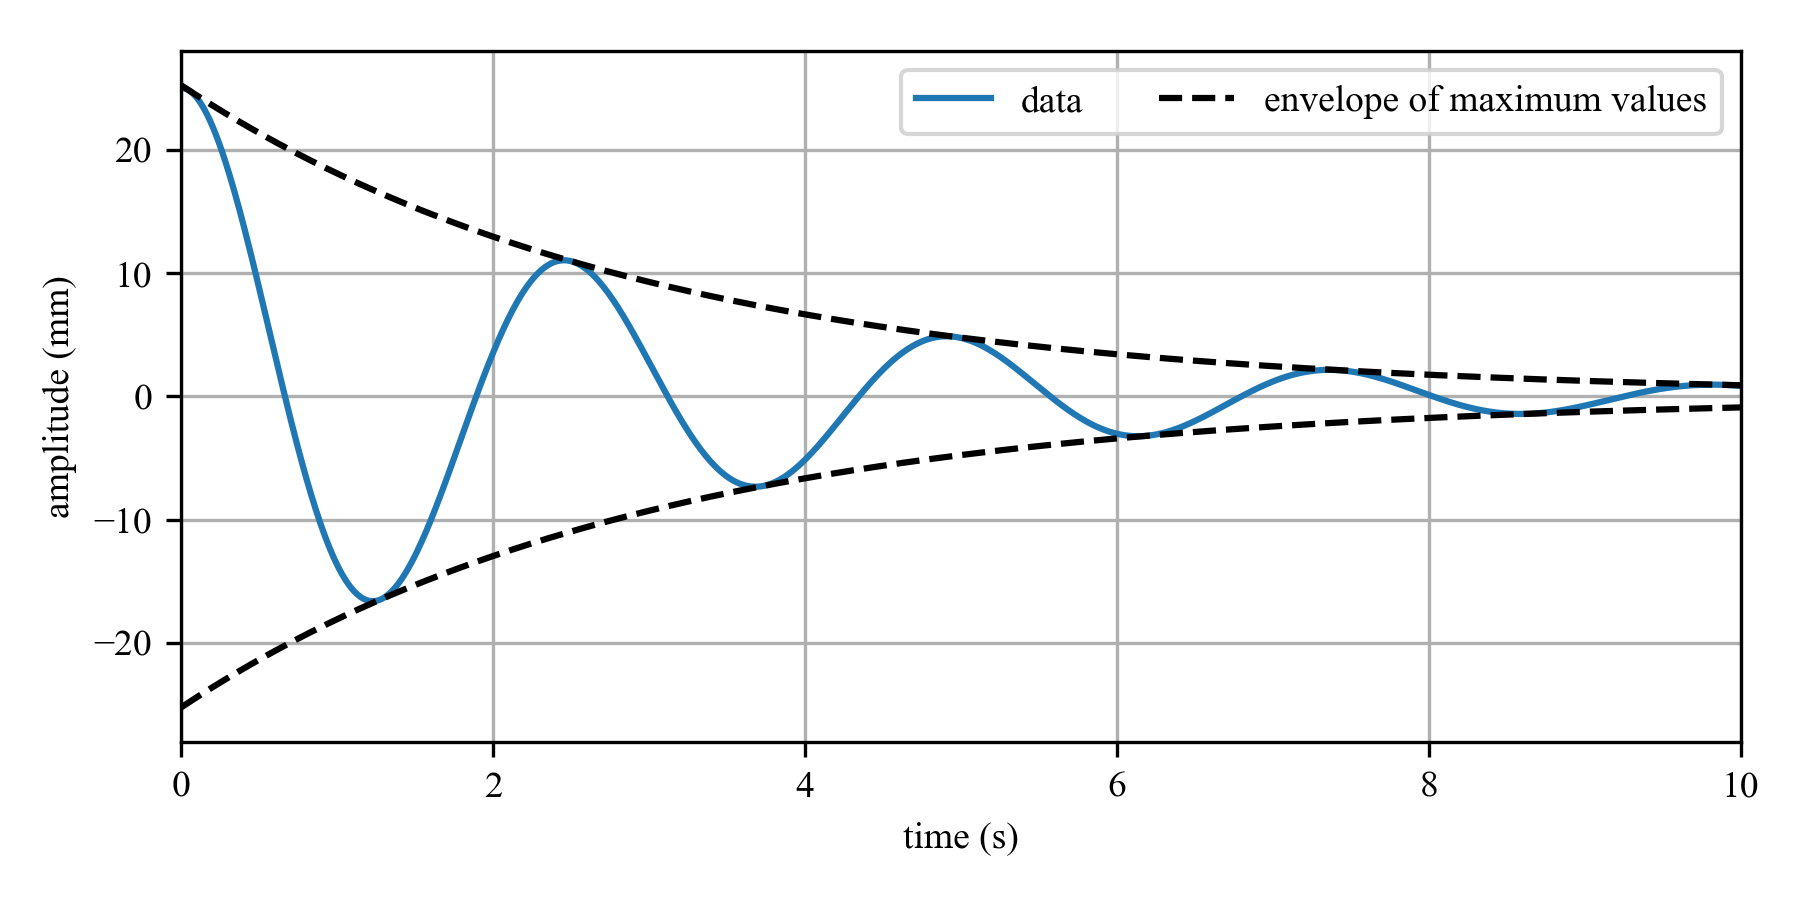
\includegraphics[]{../figures/Logarithmic_decrement.png}
				\caption{Measuring the peak displacements points in an experimental system with decay caused by damping.}
			\end{figure}
			
			\noindent we mark three points of maximum amplitude, $x_1$, $x_2$, and $x_3$ that happen at $t_1$, $t_2$, and $t_3$, respectively. Considering displacement values for the first two points $x_1$ and $x_2$. separated by a complete period ($T$).  Knowing that one cycle is $2 \pi$, the time period for this complete cycle is given by:
			\begin{equation}
				t_2-t_1 = \frac{2\pi}{\omega_d} = \frac{2\pi}{\omega_n\sqrt{1-\zeta^2}}
			\end{equation}				
			where $\omega_d$ is the damped natural frequency. This is the time period ($T$) of damped oscillations. If we derive an equation for the values of the peaks, also called the envelope of maximum values, we get: 
			\begin{equation}
				x_{\text{peaks}} = Ae^{-\zeta\omega_nt} 
			\end{equation} 		
			Knowing that the system is underdamped, $A$ can be solved for using the initial conditions $x_0$ and $v_0$, therefore: 
			\begin{equation}
				A = \frac{\sqrt{(v_0+\zeta\omega_nx_0)^2 + (x_0\omega_d)^2}}{\omega_d}
			\end{equation} 	
			In terms of $t_1$ and $t_2$, we can express the displacement at these times as:
			\begin{equation}
				x_{\text{1}} = A e^{-\zeta \omega_n t_1}
			\end{equation}				
			and 
			\begin{equation}
				x_{\text{2}} = A e^{-\zeta \omega_n t_2}
			\end{equation}		
			therefore:
			\begin{equation}
				\frac{x_{\text{1}}}{x_{\text{2}}} = \frac{e^{-\zeta \omega_n t_1}}{e^{-\zeta \omega_n t_2}} = e^{\zeta \omega_n(t_2-t_1)}
			\end{equation}		
			However, from before we know that $t_2-t_1 = \frac{2\pi}{\omega_d} = \frac{2\pi}{\omega_n\sqrt{1-\zeta^2}}$. Therefore, we can express this last equation as:
			\begin{equation}
				\frac{x_{\text{1}}}{x_{\text{2}}} =e^{\Big(\frac{2 \pi \zeta}{\sqrt{1-\zeta^2}}\Big)}
			\end{equation}			
			Next, we take the natural log of both sides to get the logarithmic decrement, denoted by $\delta$:
			\begin{equation}
				\delta = \text{ln}\bigg(\frac{x_{\text{1}}}{x_{\text{2}}}\bigg) = \text{ln}\bigg(\frac{x(t_{\text{1}})}{x(t_{\text{1}}+T)}\bigg) = \frac{2 \pi \zeta}{\sqrt{1-\zeta^2}}
			\end{equation}				
			This shows us that the ratio of any two successive amplitudes for an underdamped system, vibrating freely, is constant and is a function of the damping only. Sometimes, in experiments, it is more convenient/accurate to measure the amplitudes after say ``$n$'' peaks rather than two successive peaks (because if the damping is very small, the difference between the successive
			peaks may not be significant). The logarithmic decrement can then be given by the equation
			\begin{equation}
				\delta = \frac{1}{n}\text{ln}\bigg(\frac{x_{\text{1}}}{x_{\text{n+1}}}\bigg) =   \frac{1}{n}\text{ln}\bigg(\frac{x(t_{\text{1}})}{x(t_{\text{1}}+nT)}\bigg) = \frac{2 \pi \zeta}{\sqrt{1-\zeta^2}}
			\end{equation}				
			Once we use the experimental data to obtain $\delta$, and knowing that:
			\begin{equation}
				\delta = \frac{2 \pi \zeta}{\sqrt{1-\zeta^2}}
			\end{equation}	
			we can calculate the value of $\zeta$:
			\begin{equation}
				\zeta = \frac{\delta}{\sqrt{4\pi^2+\delta^2}}
			\end{equation}
			Therefore, having $\zeta$ we can solve for the coefficient of damping, $c$, as: 
			\begin{equation}
				c = \zeta 2\sqrt{km}
			\end{equation}					

\begin{example}
			
			Calculate the damping coefficient for the system with the measured amplitude as expressed below given that $m$ = 3 kg and $k$ = 43 N/m. Use $t_1$ = 1 sec, and $t_{n+1} =t_4=6$ sec.

			\begin{figure}[H]
				\centering
				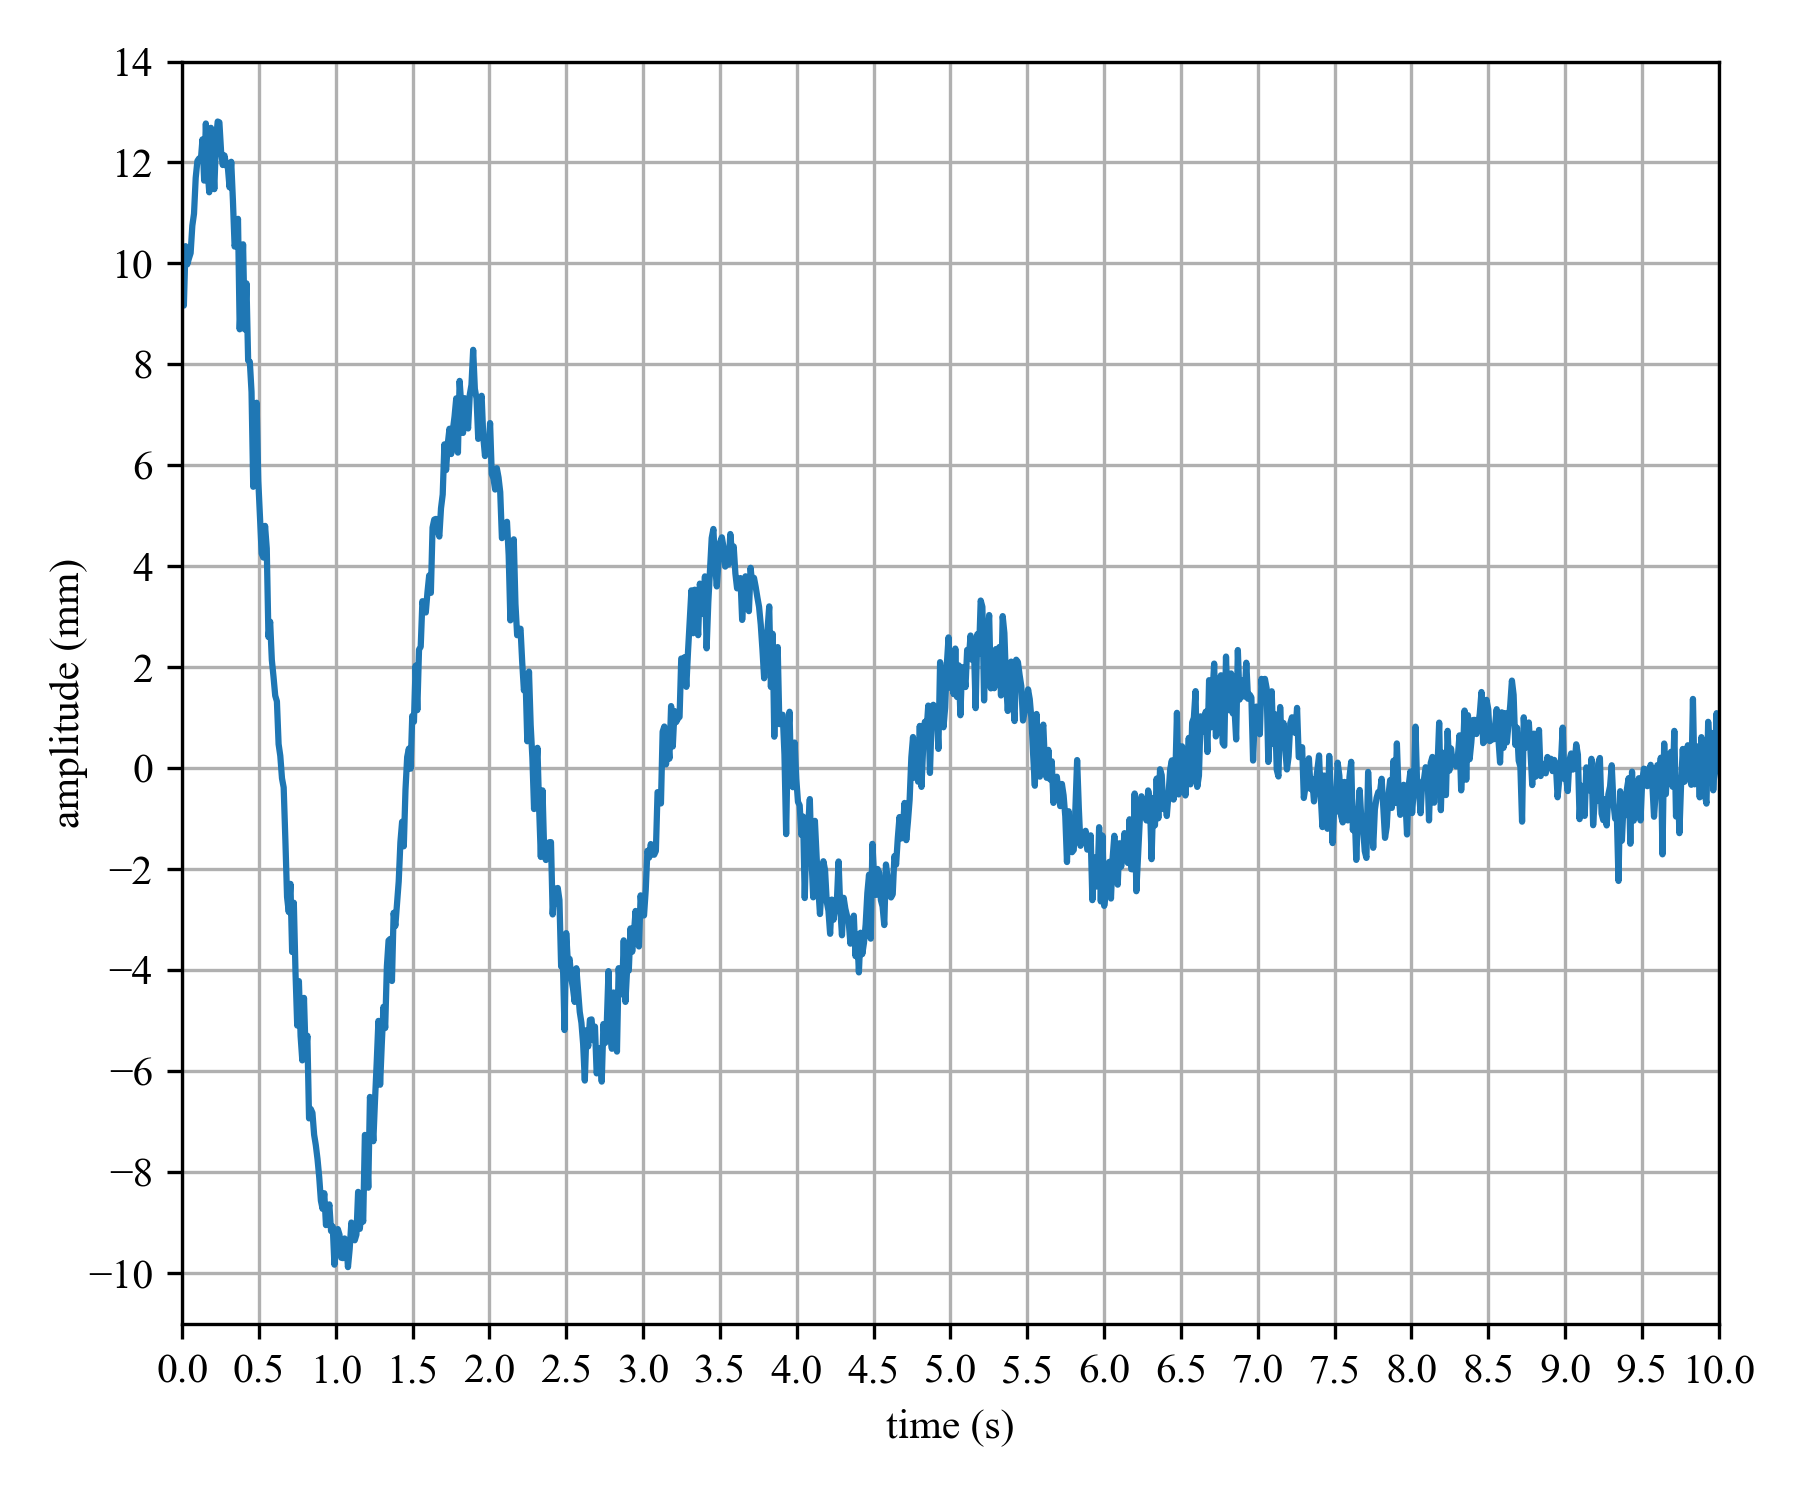
\includegraphics[]{../figures/Logarithmic_decrement_with_noise.png}
				\caption{Response from an experimental system with noise.}
			\end{figure}
			
			\noindent\textbf{Solution:} 
						
			First, from the plot we can determine that $x_1=-9.5$ mm and $x_3=-1.8$ mm where $n=3$. Thereafter, we can solve for $\delta$:  
			\begin{equation}
				\delta = \frac{1}{3}\text{ln}\bigg(\frac{x_{\text{1}}}{x_{\text{4}}}\bigg) = \frac{1}{3}\text{ln}\bigg(\frac{-9.5}{-1.8}\bigg) = 0.554
			\end{equation}						
			Next, we can calculate $\zeta$, as: 
			\begin{equation}
				\zeta = \frac{\delta}{\sqrt{4\pi^2+\delta^2}} = \frac{0.554}{\sqrt{4\pi^2+0.554^2}} = 0.0879
			\end{equation}
			And lastly:			
			\begin{equation}
				c = \zeta 2\sqrt{km} = 0.0879 \cdot 2\sqrt{43 \cdot 3} = 2.0 \text{ kg/s}
			\end{equation}	

\end{example}

	
\begin{example}
			
			The free response of a 1000-kg automobile with a stiffness of $k$ = 400,000 N/m is observed to be underdamped. Modeling the automobile as a single-degree-of-freedom oscillation in the vertical direction, as annotated in figure \ref{fig:vehicle_wheel_undamped}, determine the damping coefficient if the displacement at $t_1$ is measured to be 2 cm and 0.22 cm at $t_2$.

			\noindent\textbf{Solution:} 
						
			Knowing $x_1$ = 2 cm and $x_2$ = 0.22 cm and $t_2 = T + t_1$, therefore:
			\begin{equation}
				\delta = \text{ln}\frac{x_1}{x_2} = \text{ln}\frac{2}{0.22} = 2.207
			\end{equation}			
			and:
			\begin{equation}
				\zeta = \bigg(\frac{\delta}{\sqrt{4\pi^2+\delta^2}}\bigg) = \bigg(\frac{2.207}{\sqrt{4\pi^2+2.207^2}}\bigg) = 0.331
			\end{equation}
			therefore, we can obtain the damping coefficient as
			\begin{equation}
				c = 2\zeta\sqrt{km}=2(0.331)\sqrt{400,000 \cdot 1,000} = 13,256 \hspace{1ex} 
				\text{kg/s} 
			\end{equation}	

\end{example}
		
						
			
			


\end{document}